\subsubsection{EVEN and ODD} \label{sssec:skipp}

In Figs. \ref{fig:Hval_Even} and \ref{fig:Hval_Odd} we can see that quantifiers related to the normalized histogram of values slightly degrades with the skipping procedure.
For example $\left\langle H_{hist}\right\rangle $ reduces from $0.9722$ without skipping to $0.9459$ for EVEN and $0.9706$ for ODD. 
This difference between EVEN and ODD in floating point is because a high dispersion was obtained for $H_{hist}$, $H_{BP}$ and $C_{BP}$ but not for $H_{BPW}$ or $C_{BPW}$.

Figures \ref{fig:Hbp_Even} to \ref{fig:MP_Even} and Figs. \ref{fig:Hbp_Odd} to \ref{fig:MP_Odd} show the results of BP and BPW quantifiers for EVEN and ODD respectively.
Higher accuracy is required to achieve lower complexity than without using skipping.
From the MP point of view a great improvement is obtained using any of the skipping strategies but ODD is slightly better than EVEN.
Missing patterns are reduced to $MP = 118$ for EVEN and ODD, increasing the maximum allowed Bandt \& Pompe entropy that reaches the mean value $\left\langle H_{BP}\right\rangle  = 0.8381$ for EVEN, and $\left\langle H_{BP}\right\rangle  = 0.9094$.
The complexity is reduced to $\left\langle C_{BP}\right\rangle = 0.224$ for EVEN and $\left\langle C_{BP}\right\rangle = 0.282$ for ODD.
The minimum number of bits to converge to this value is $B>40$ for both EVEN and ODD maps.

\begin{figure}[H]
	\centering
	\begin{subfigure}[b]{0.49\textwidth}
		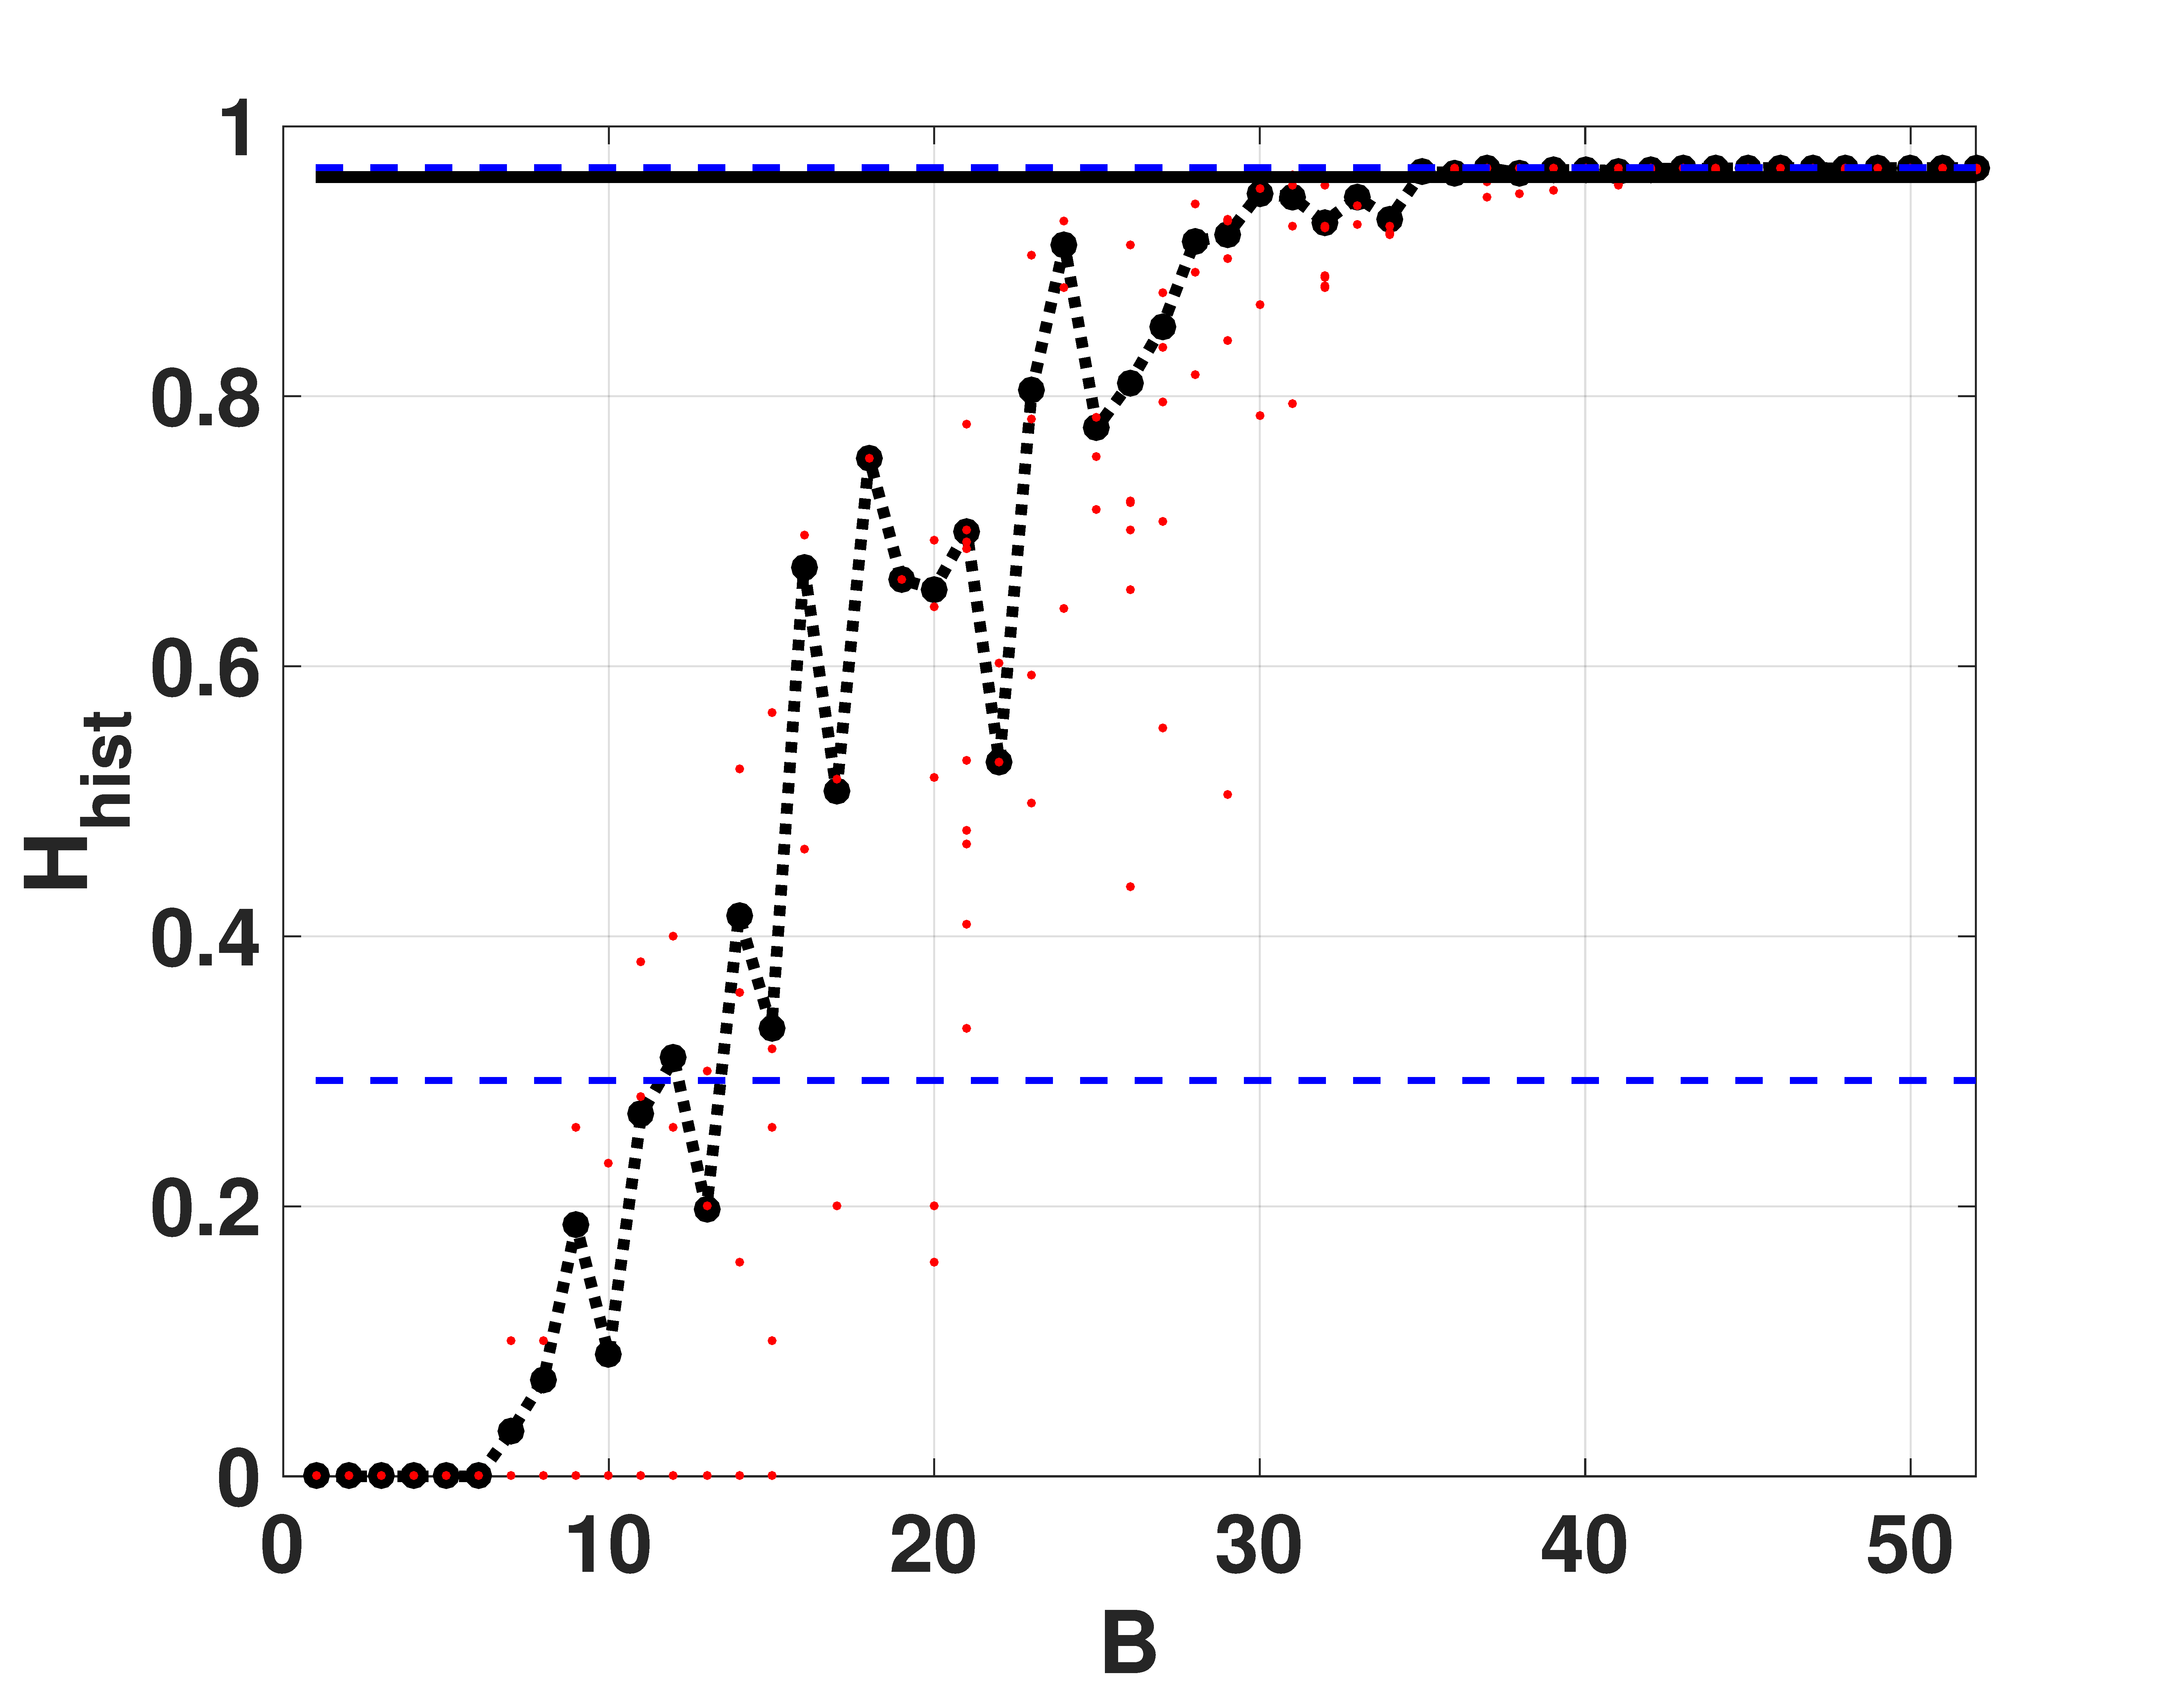
\includegraphics[width=\textwidth]{Hval_Even}
		\caption{$H_{hist}$ vs. $B$}
		\label{fig:Hval_Even}
	\end{subfigure}
	\begin{subfigure}[b]{0.49\textwidth}
		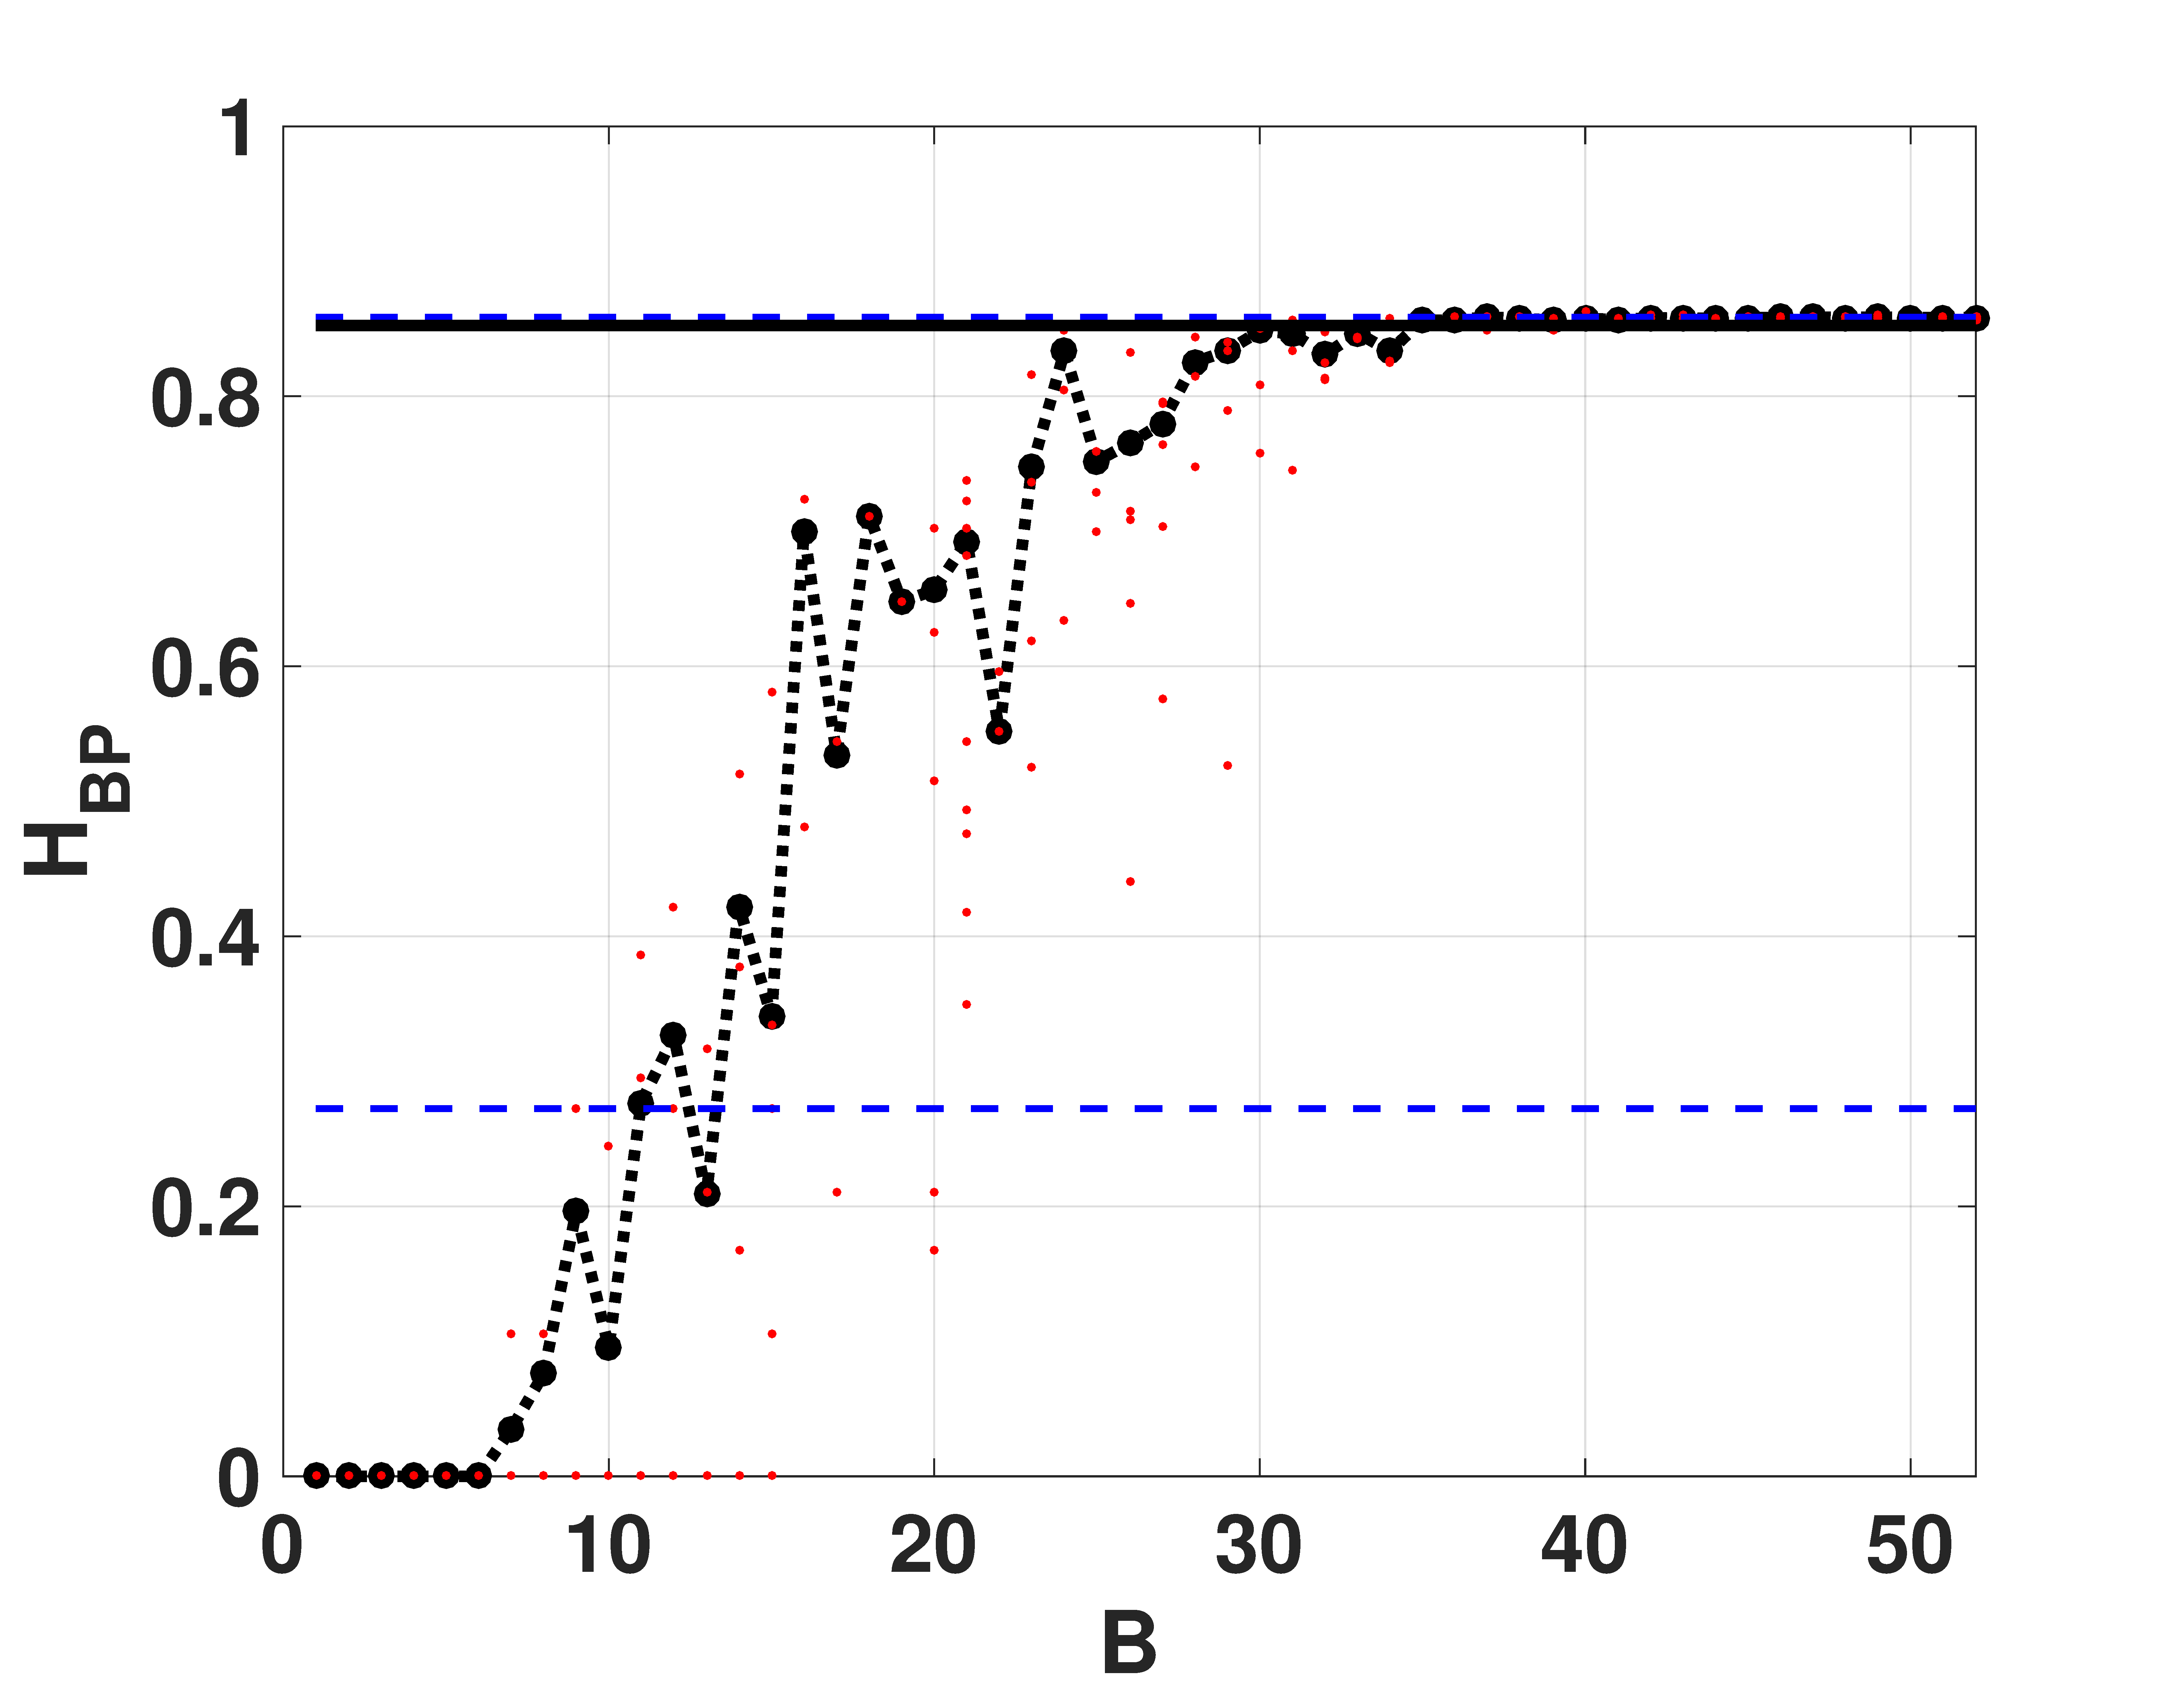
\includegraphics[width=\textwidth]{Hbp_Even}
		\caption{$H_{BP}$ vs. $B$}
		\label{fig:Hbp_Even}
	\end{subfigure}
	\begin{subfigure}[b]{0.49\textwidth}
		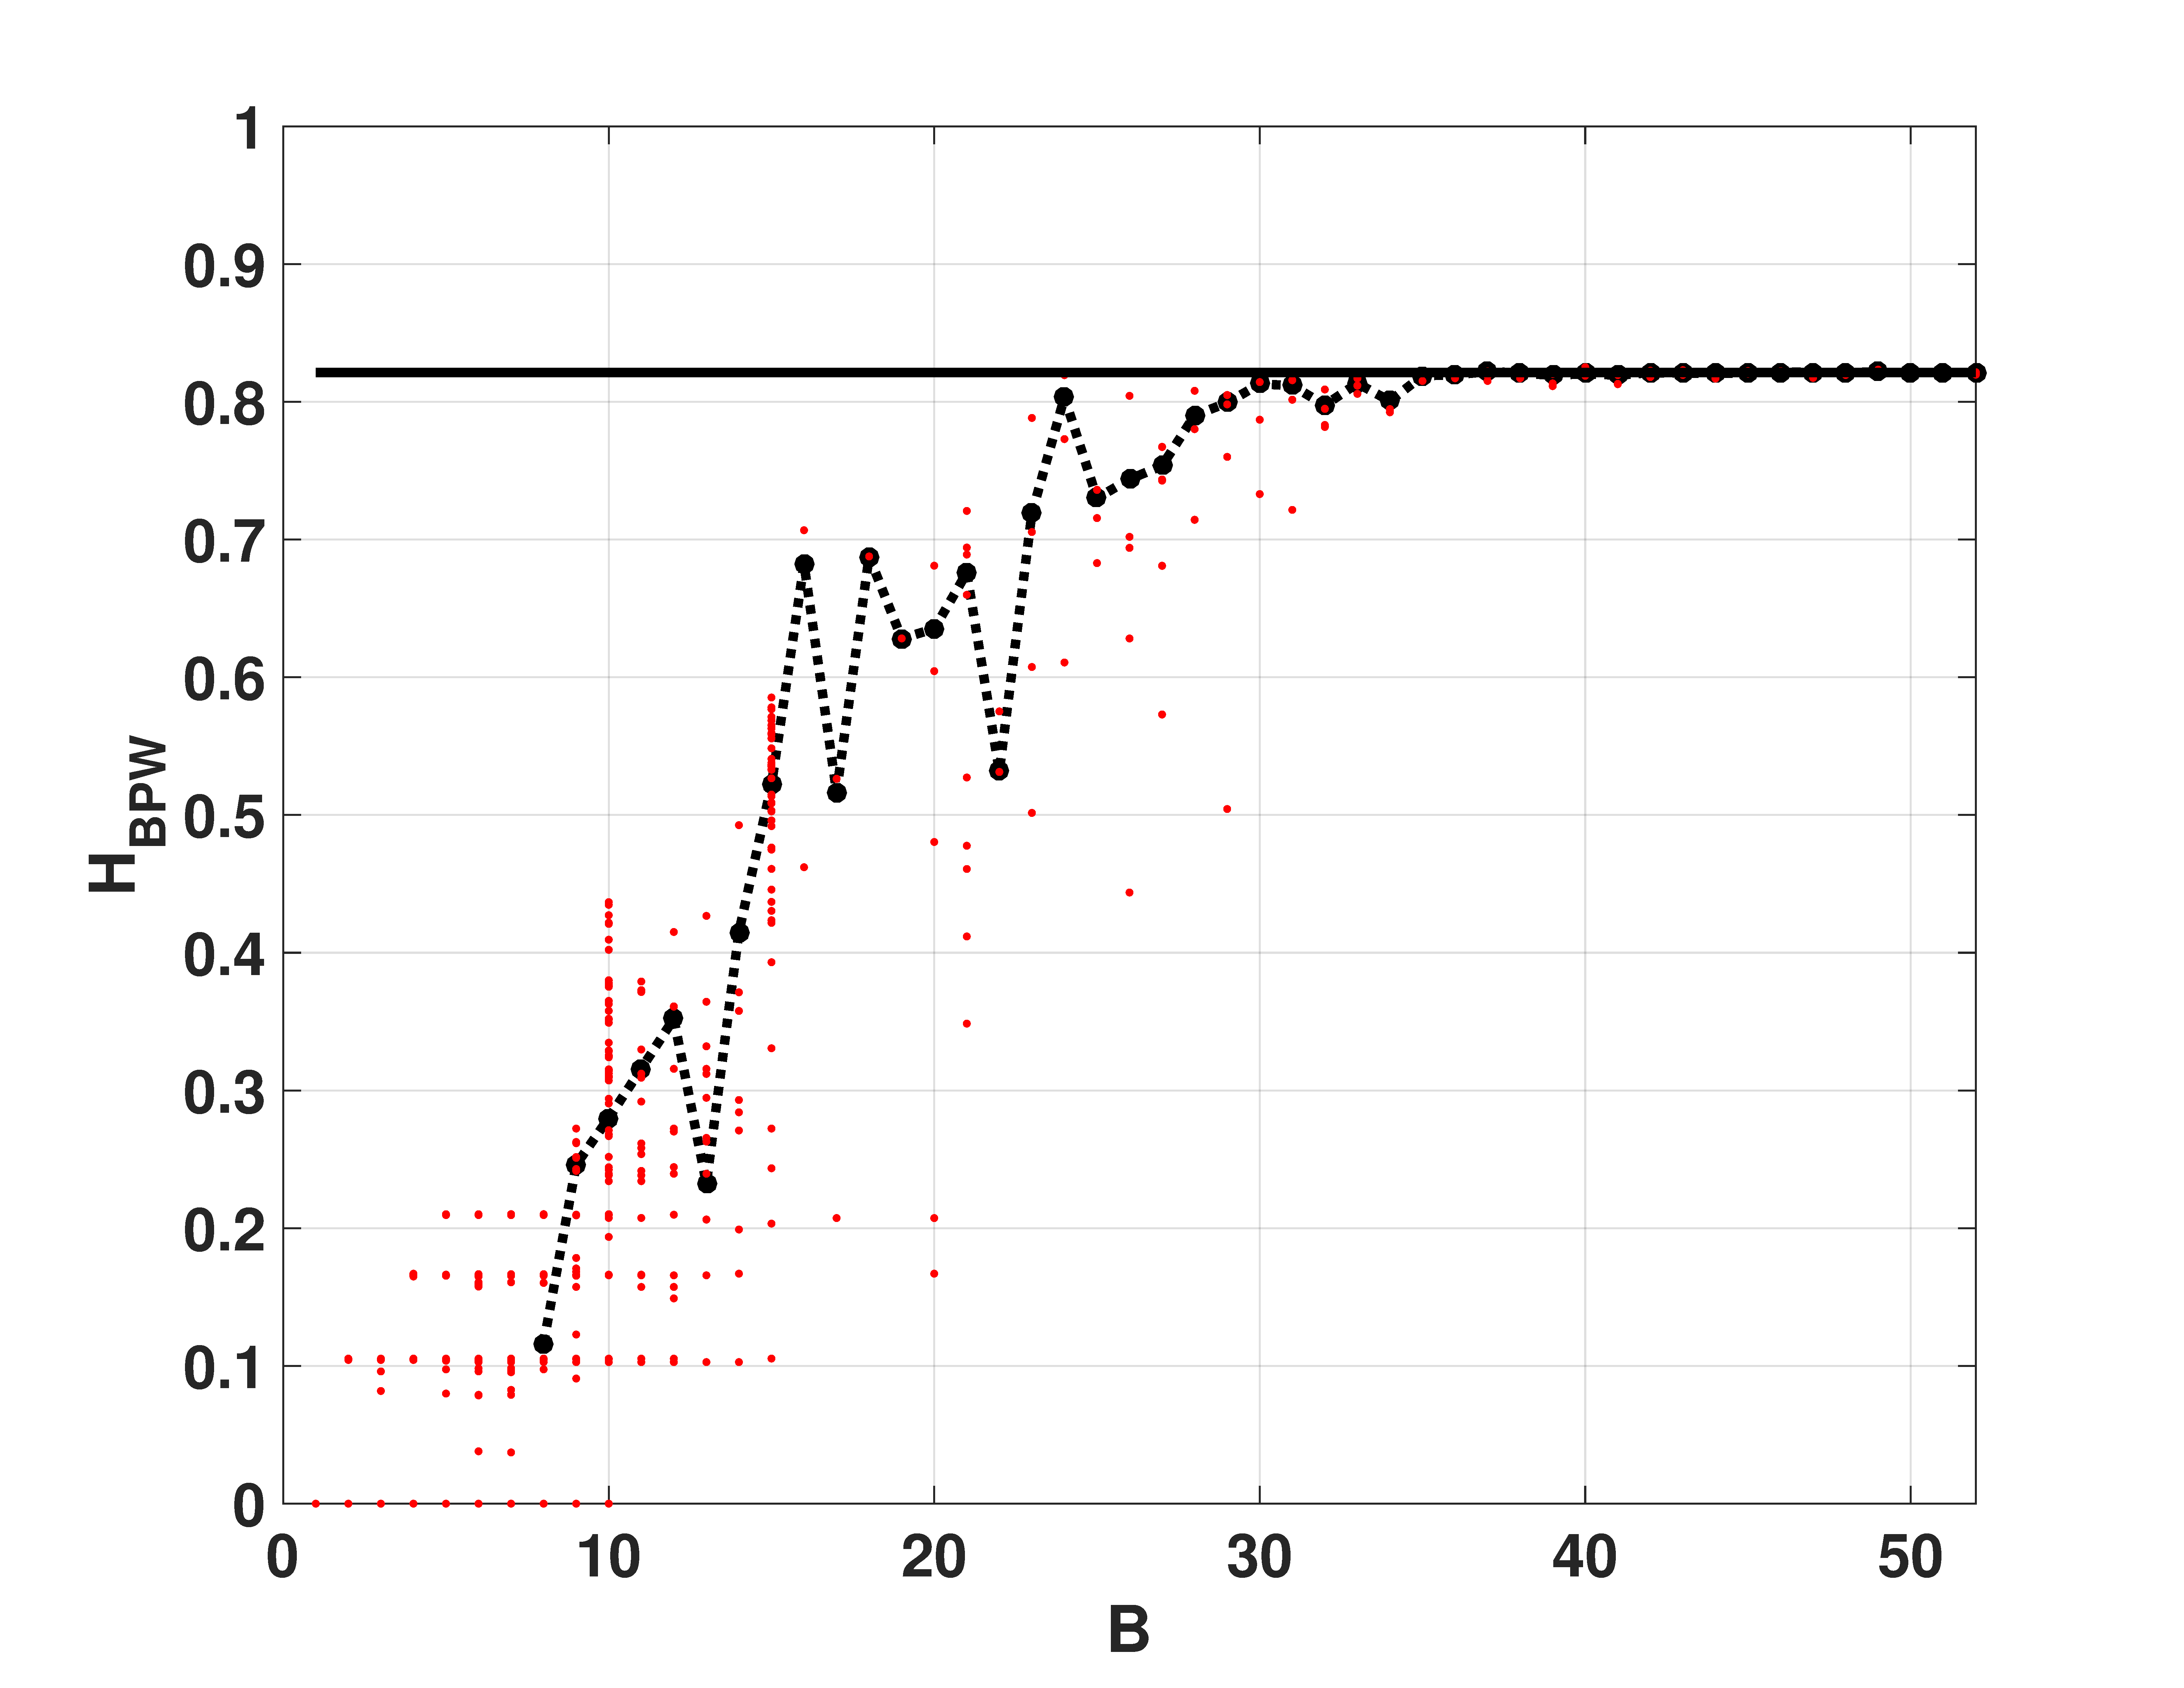
\includegraphics[width=\textwidth]{Hbpw_Even}
		\caption{$H_{BPW}$ vs. $B$}
		\label{fig:Hbpw_Even}
	\end{subfigure}
	\begin{subfigure}[b]{0.49\textwidth}
		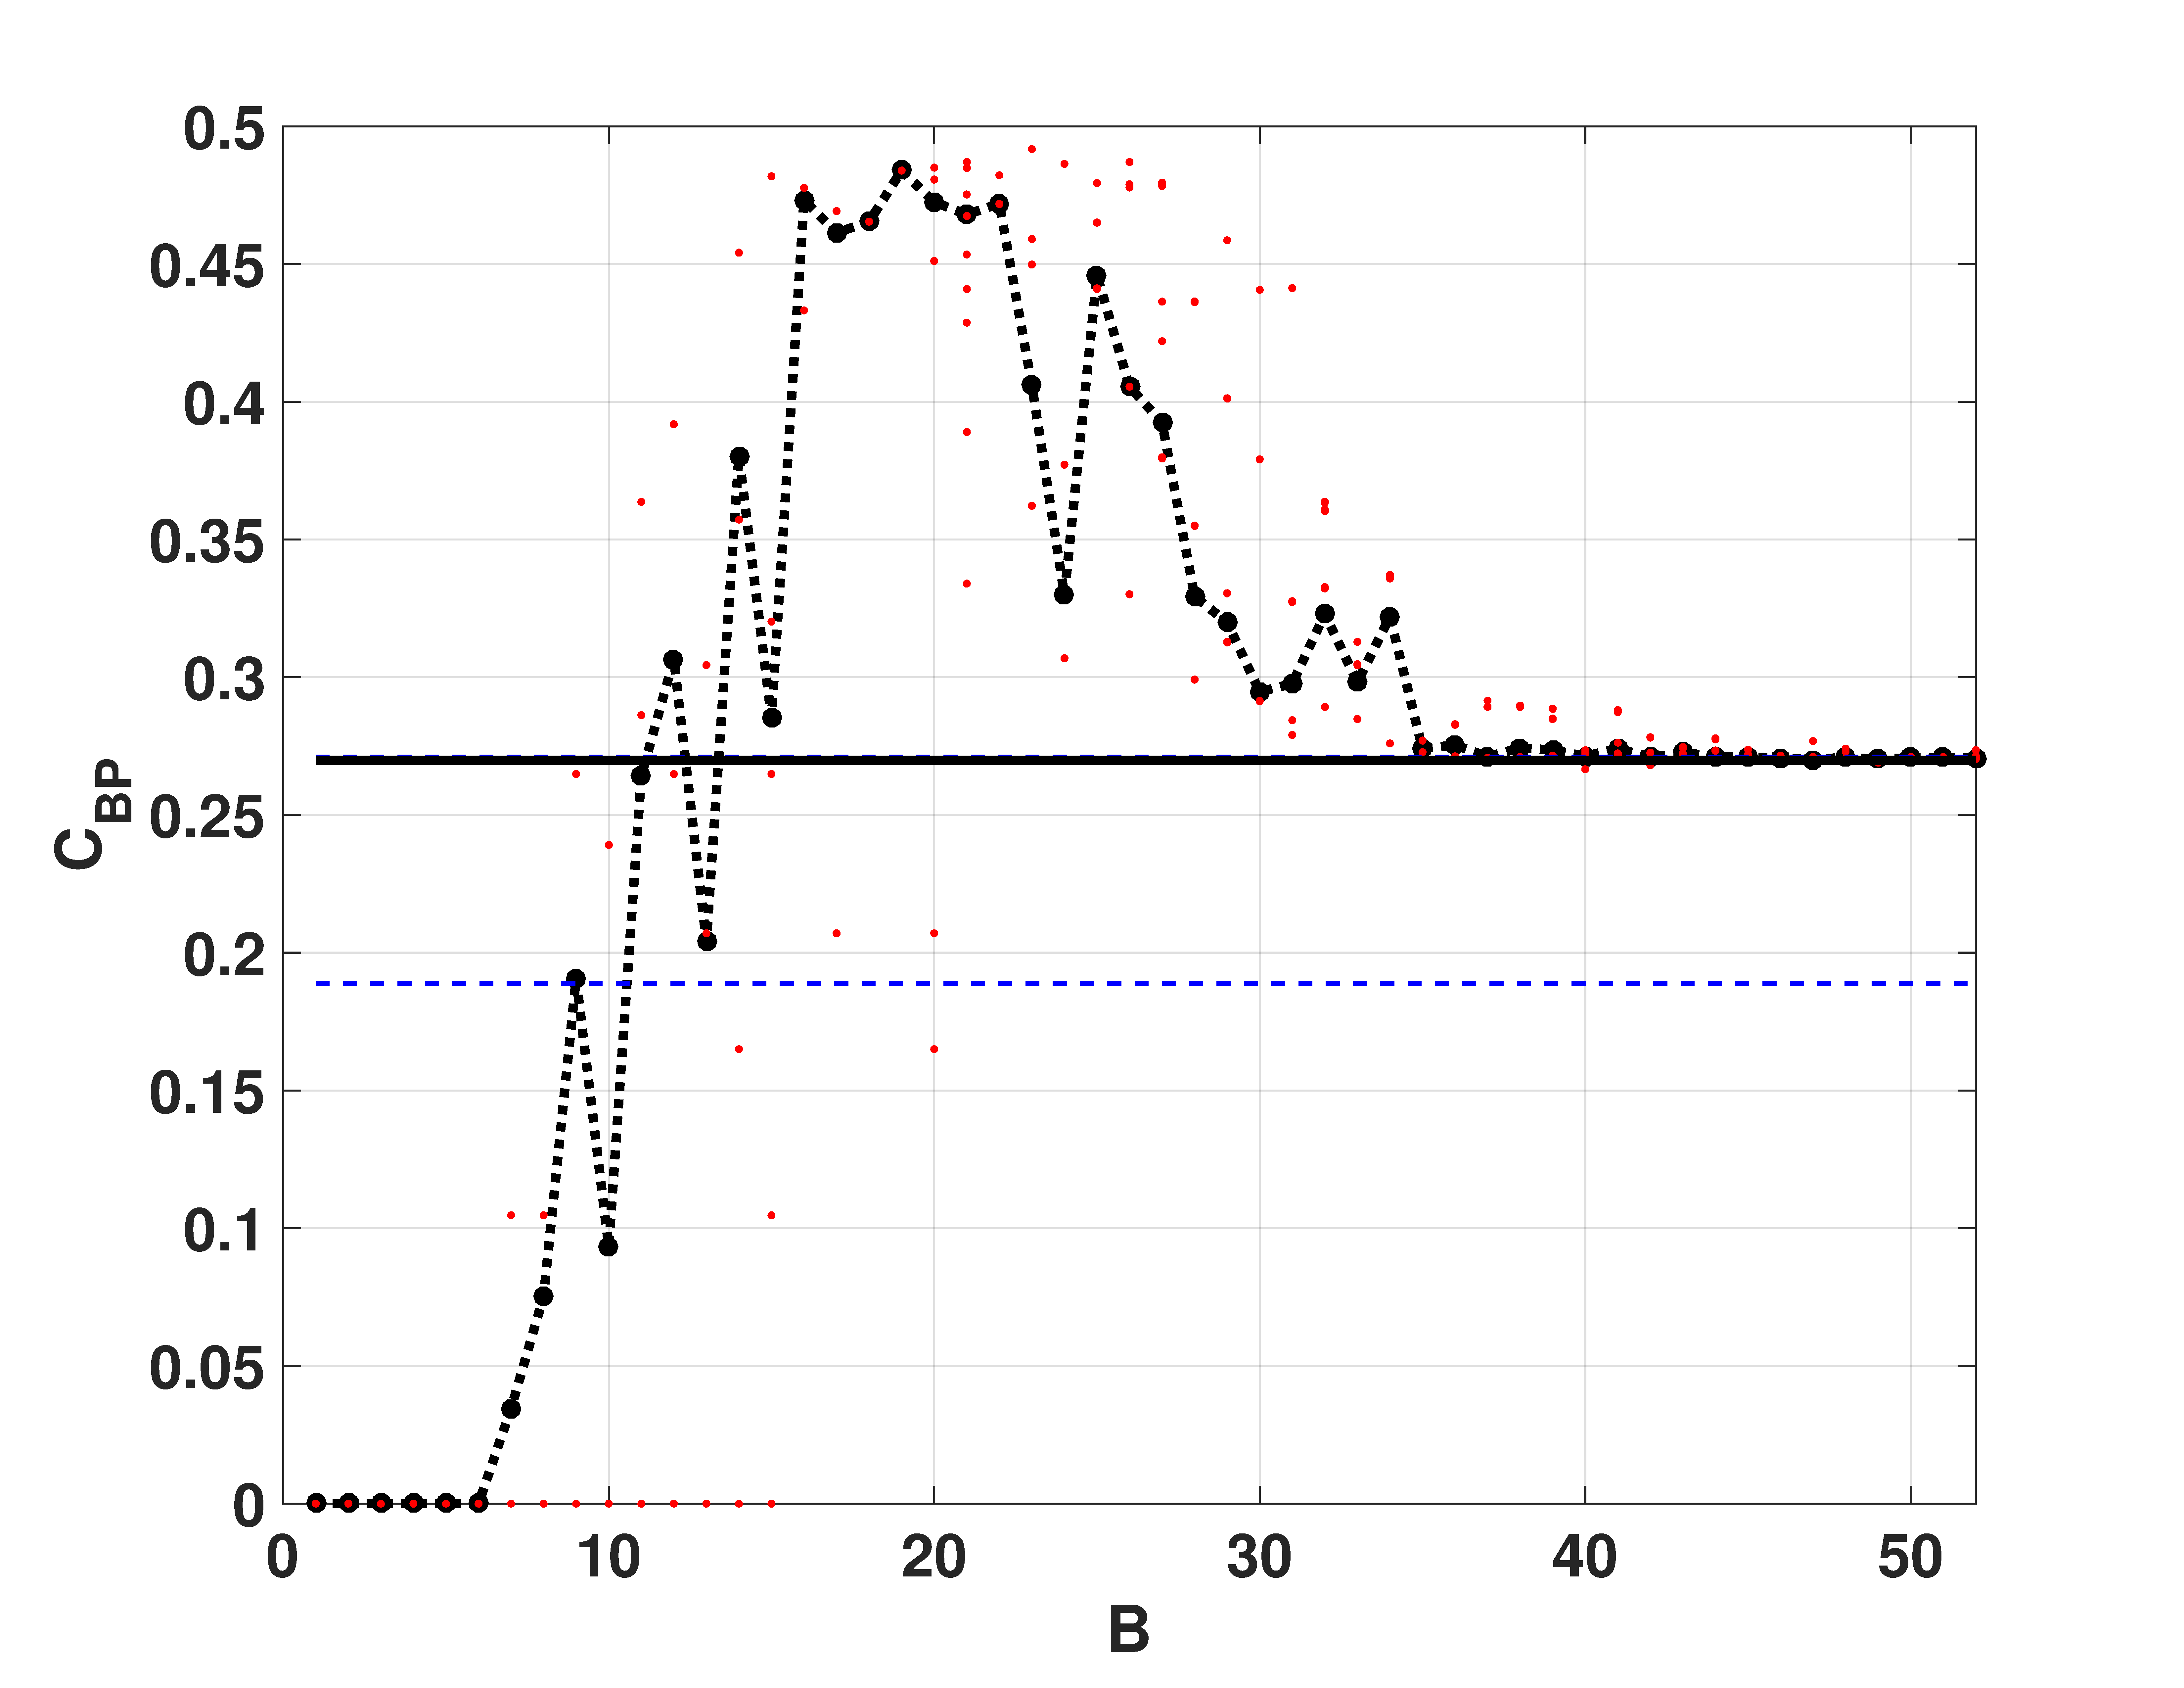
\includegraphics[width=\textwidth]{Cbp_Even}
		\caption{$C_{BP}$ vs. $B$}
		\label{fig:Cbp_Even}
	\end{subfigure}
	\begin{subfigure}[b]{0.49\textwidth}
		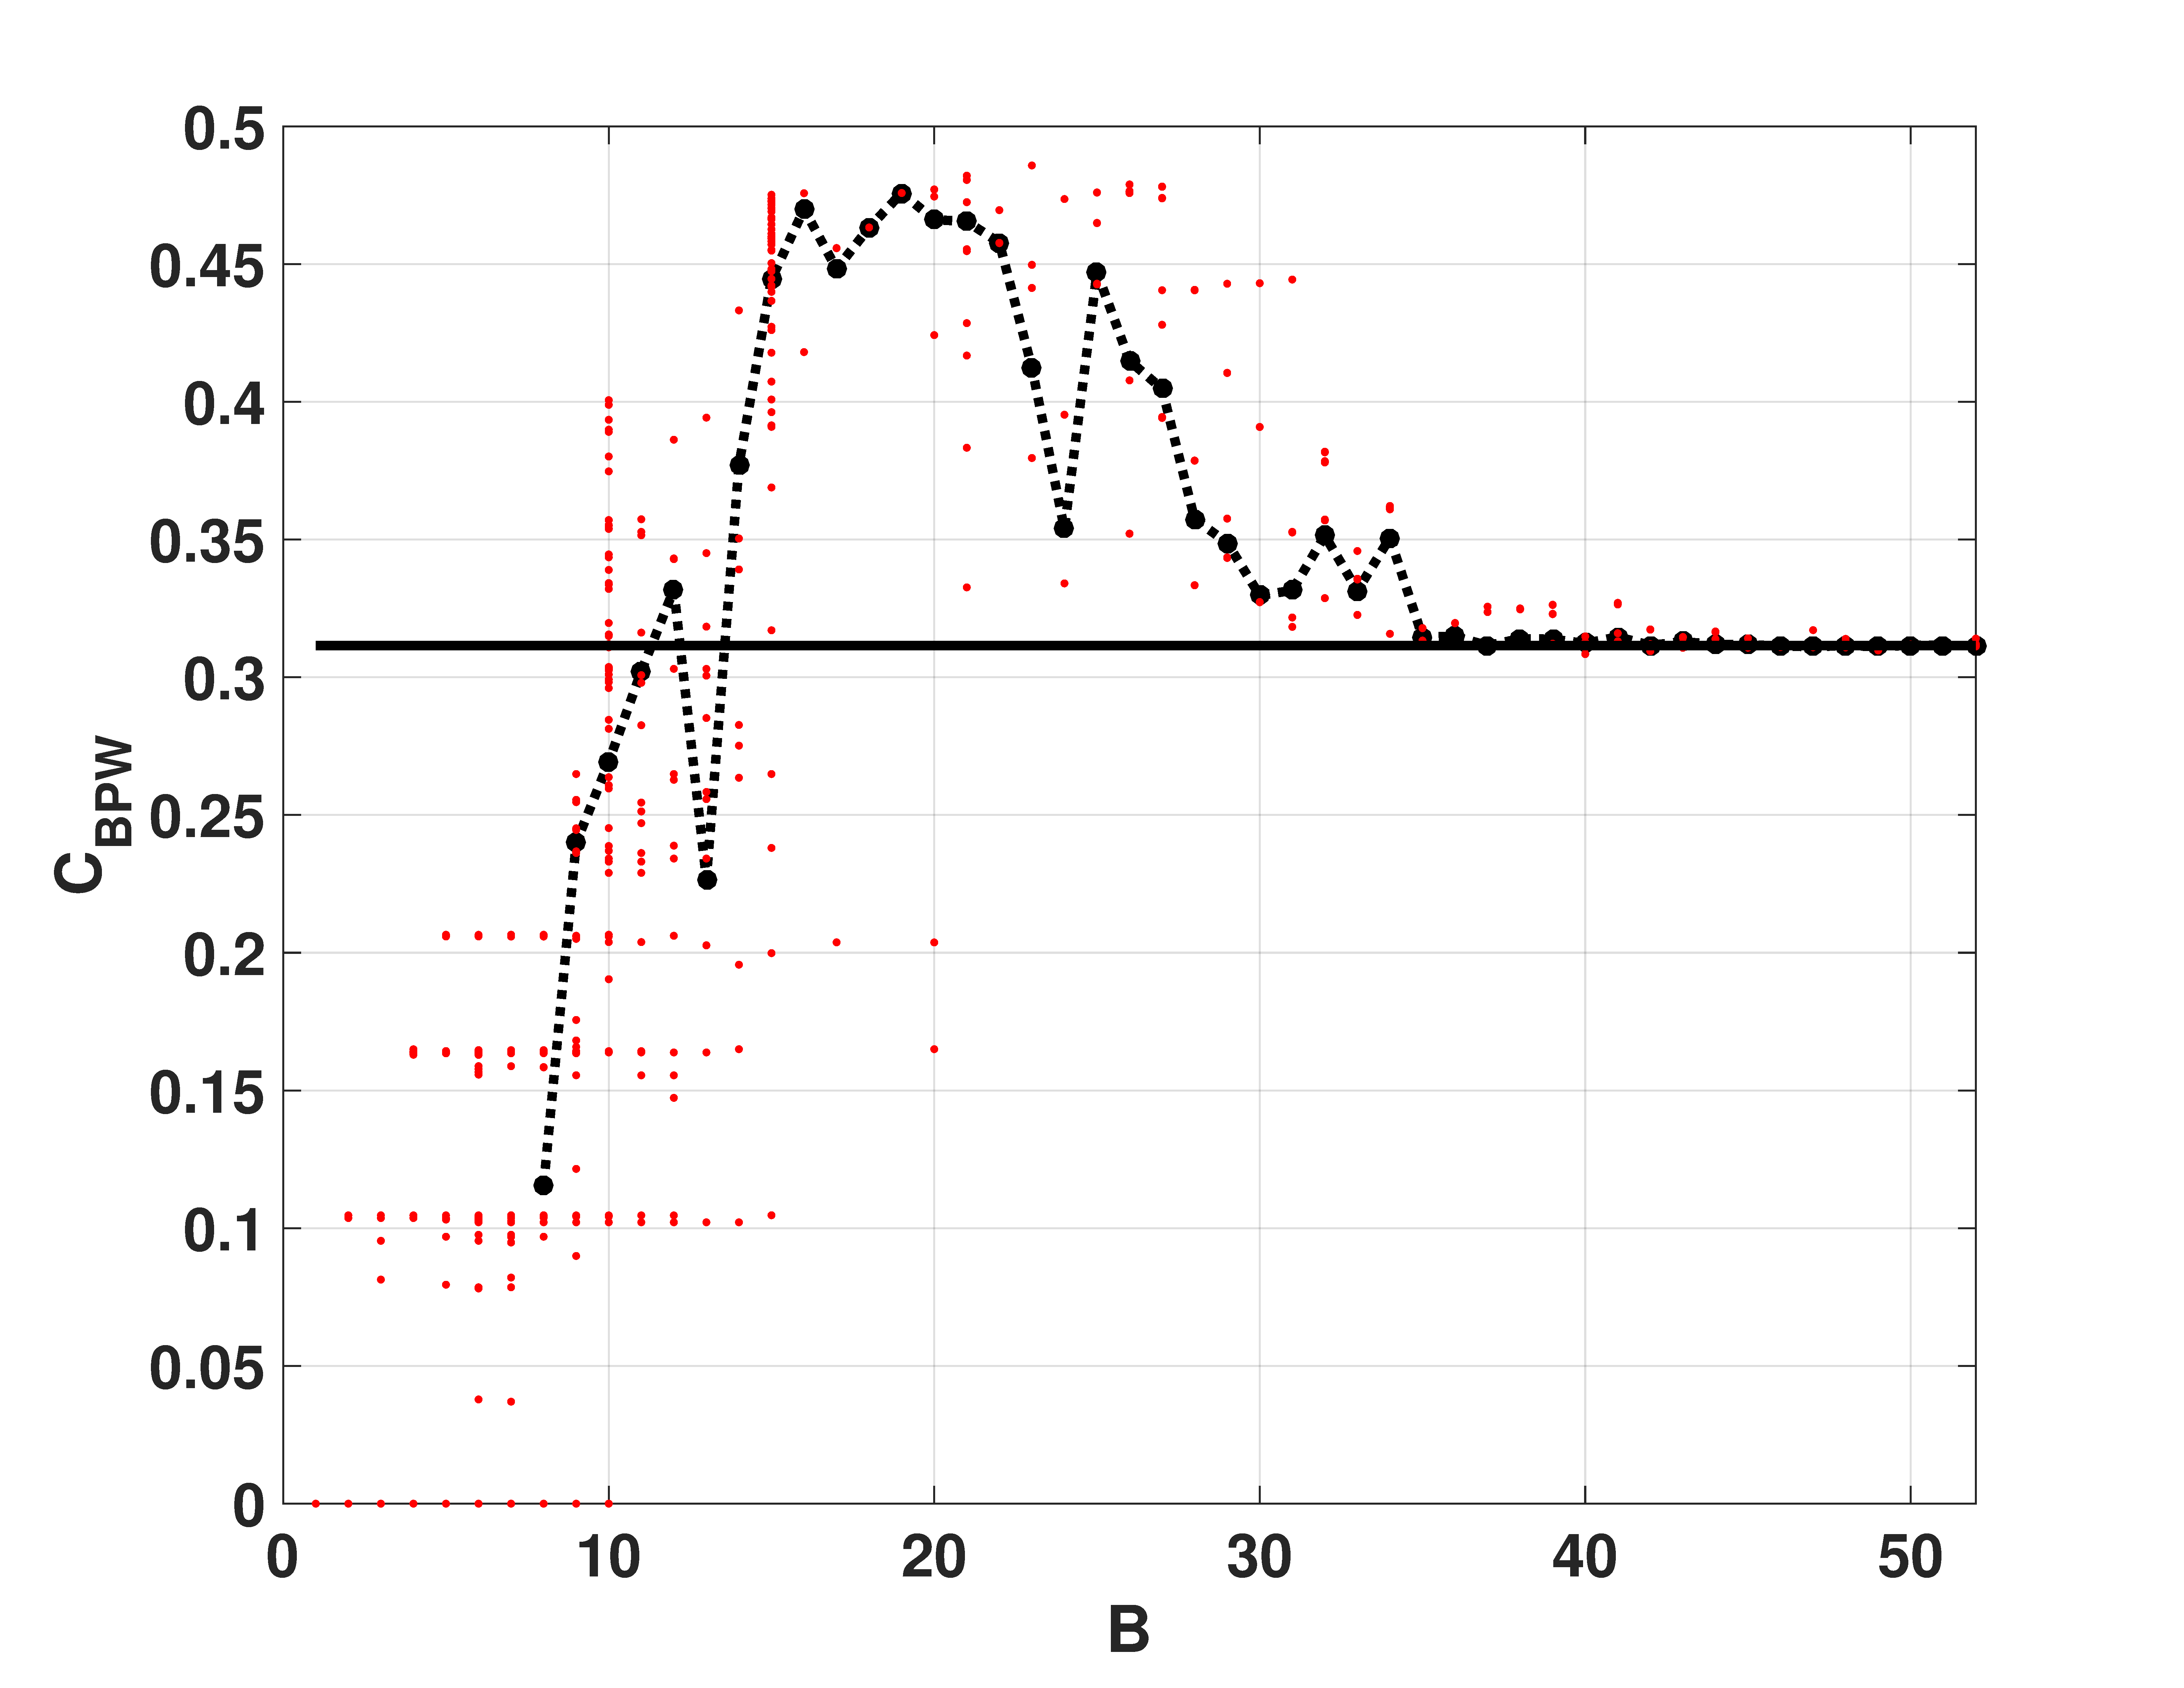
\includegraphics[width=\textwidth]{Cbpw_Even}
		\caption{$C_{BPW}$ vs. $B$}
		\label{fig:Cbpw_Even}
	\end{subfigure}
	\begin{subfigure}[b]{0.49\textwidth}
		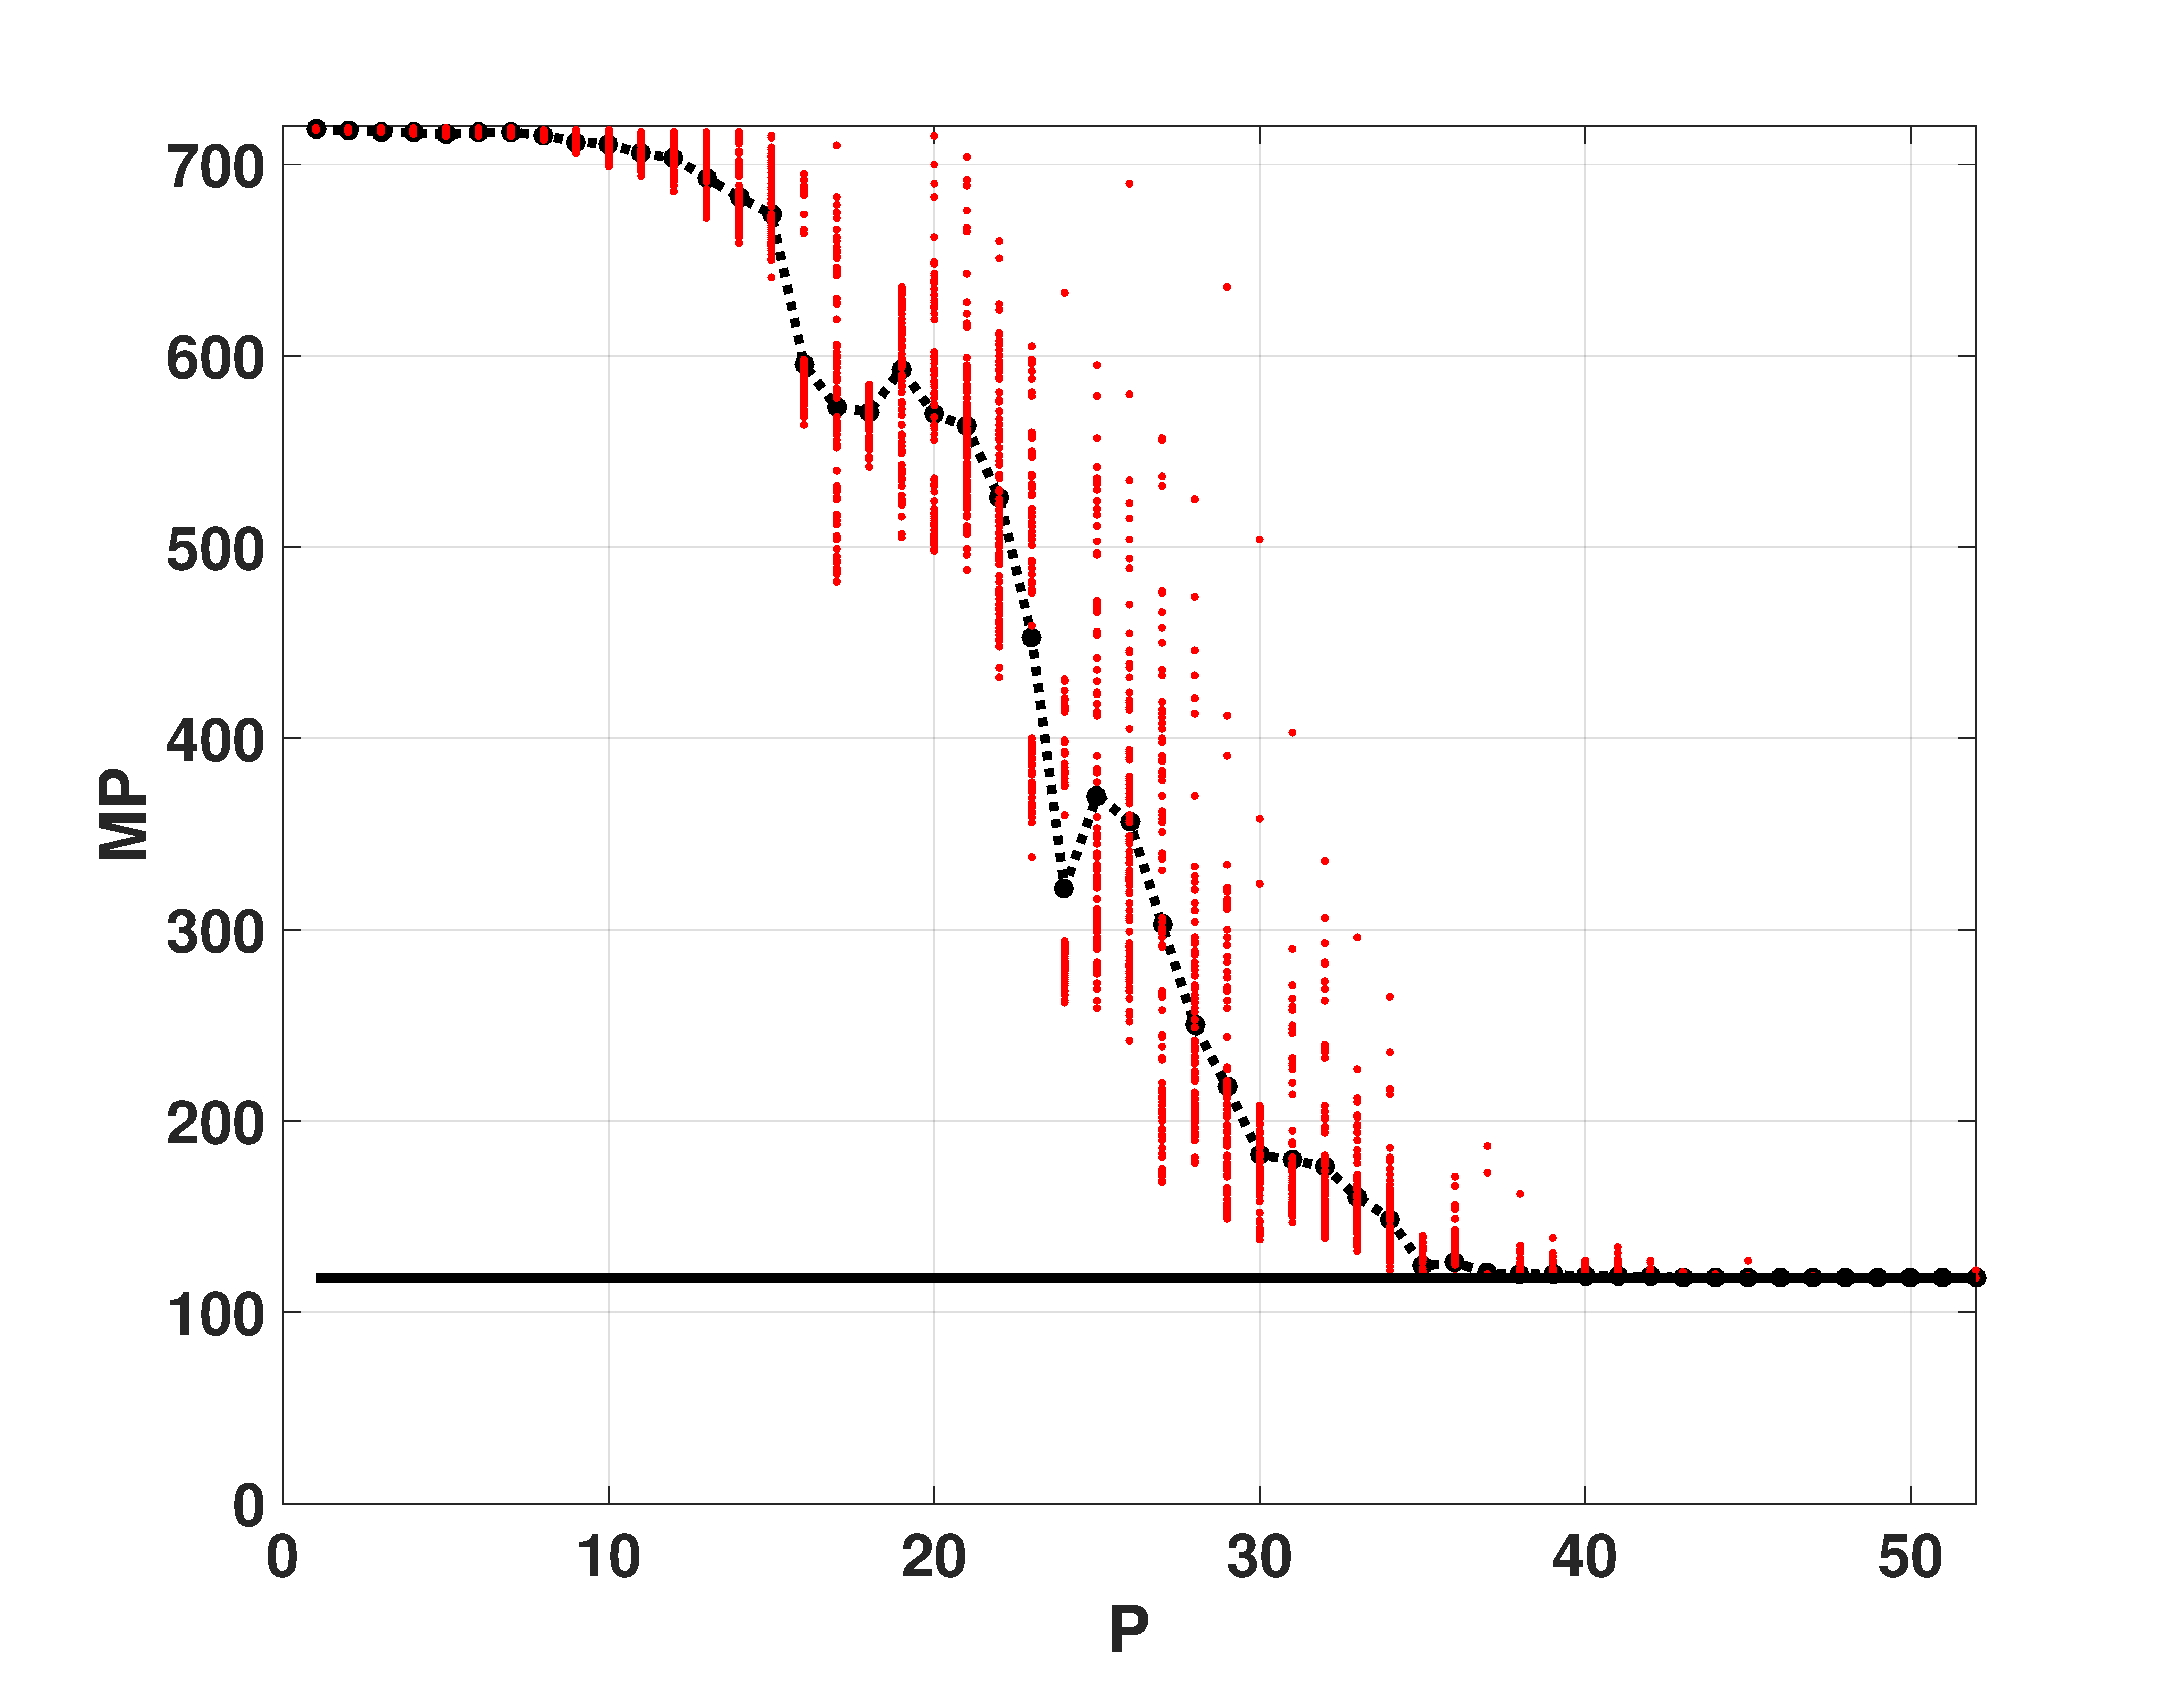
\includegraphics[width=\textwidth]{MP_Even}
		\caption{MP vs. $B$}
		\label{fig:MP_Even}
	\end{subfigure}
	\caption{Statistical properties of EVEN map.}
	\label{fig:EVEN_QuantiB}
\end{figure}

\begin{figure}[H]
	\centering
	\begin{subfigure}[b]{0.49\textwidth}
		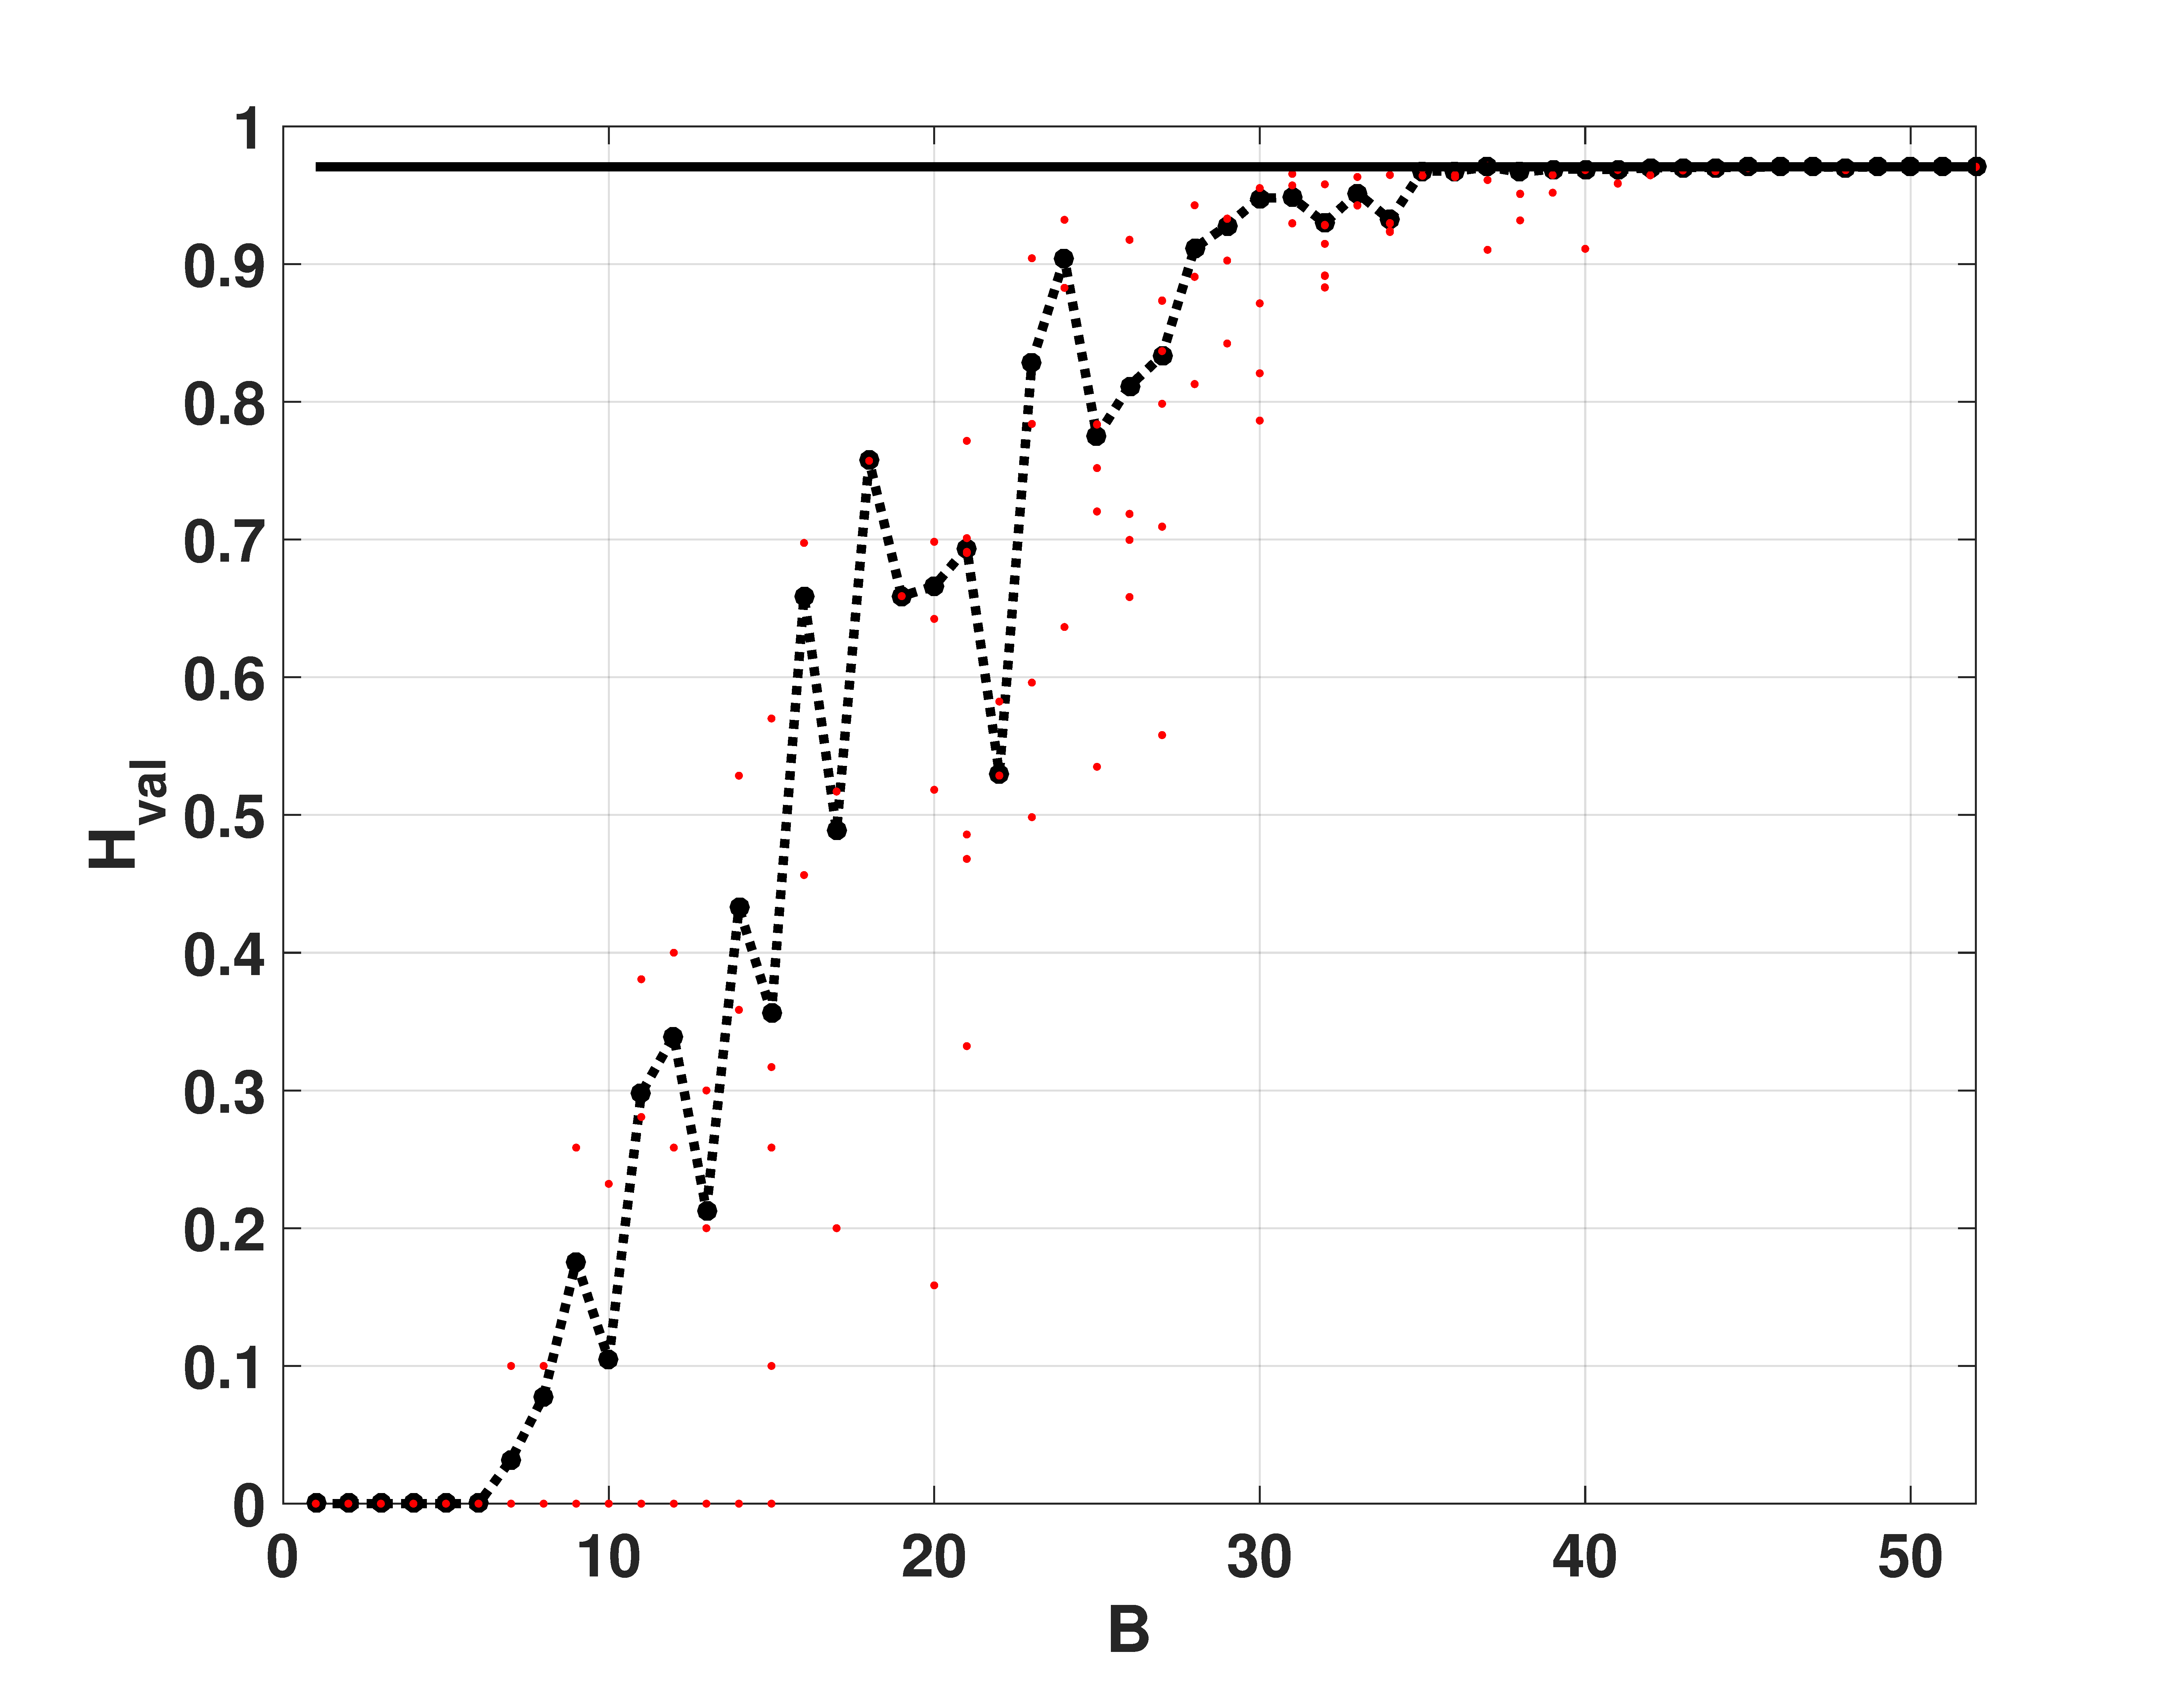
\includegraphics[width=\textwidth]{Hval_Odd}
		\caption{$H_{hist}$ vs. $B$}
		\label{fig:Hval_Odd}
	\end{subfigure}
	\begin{subfigure}[b]{0.49\textwidth}
		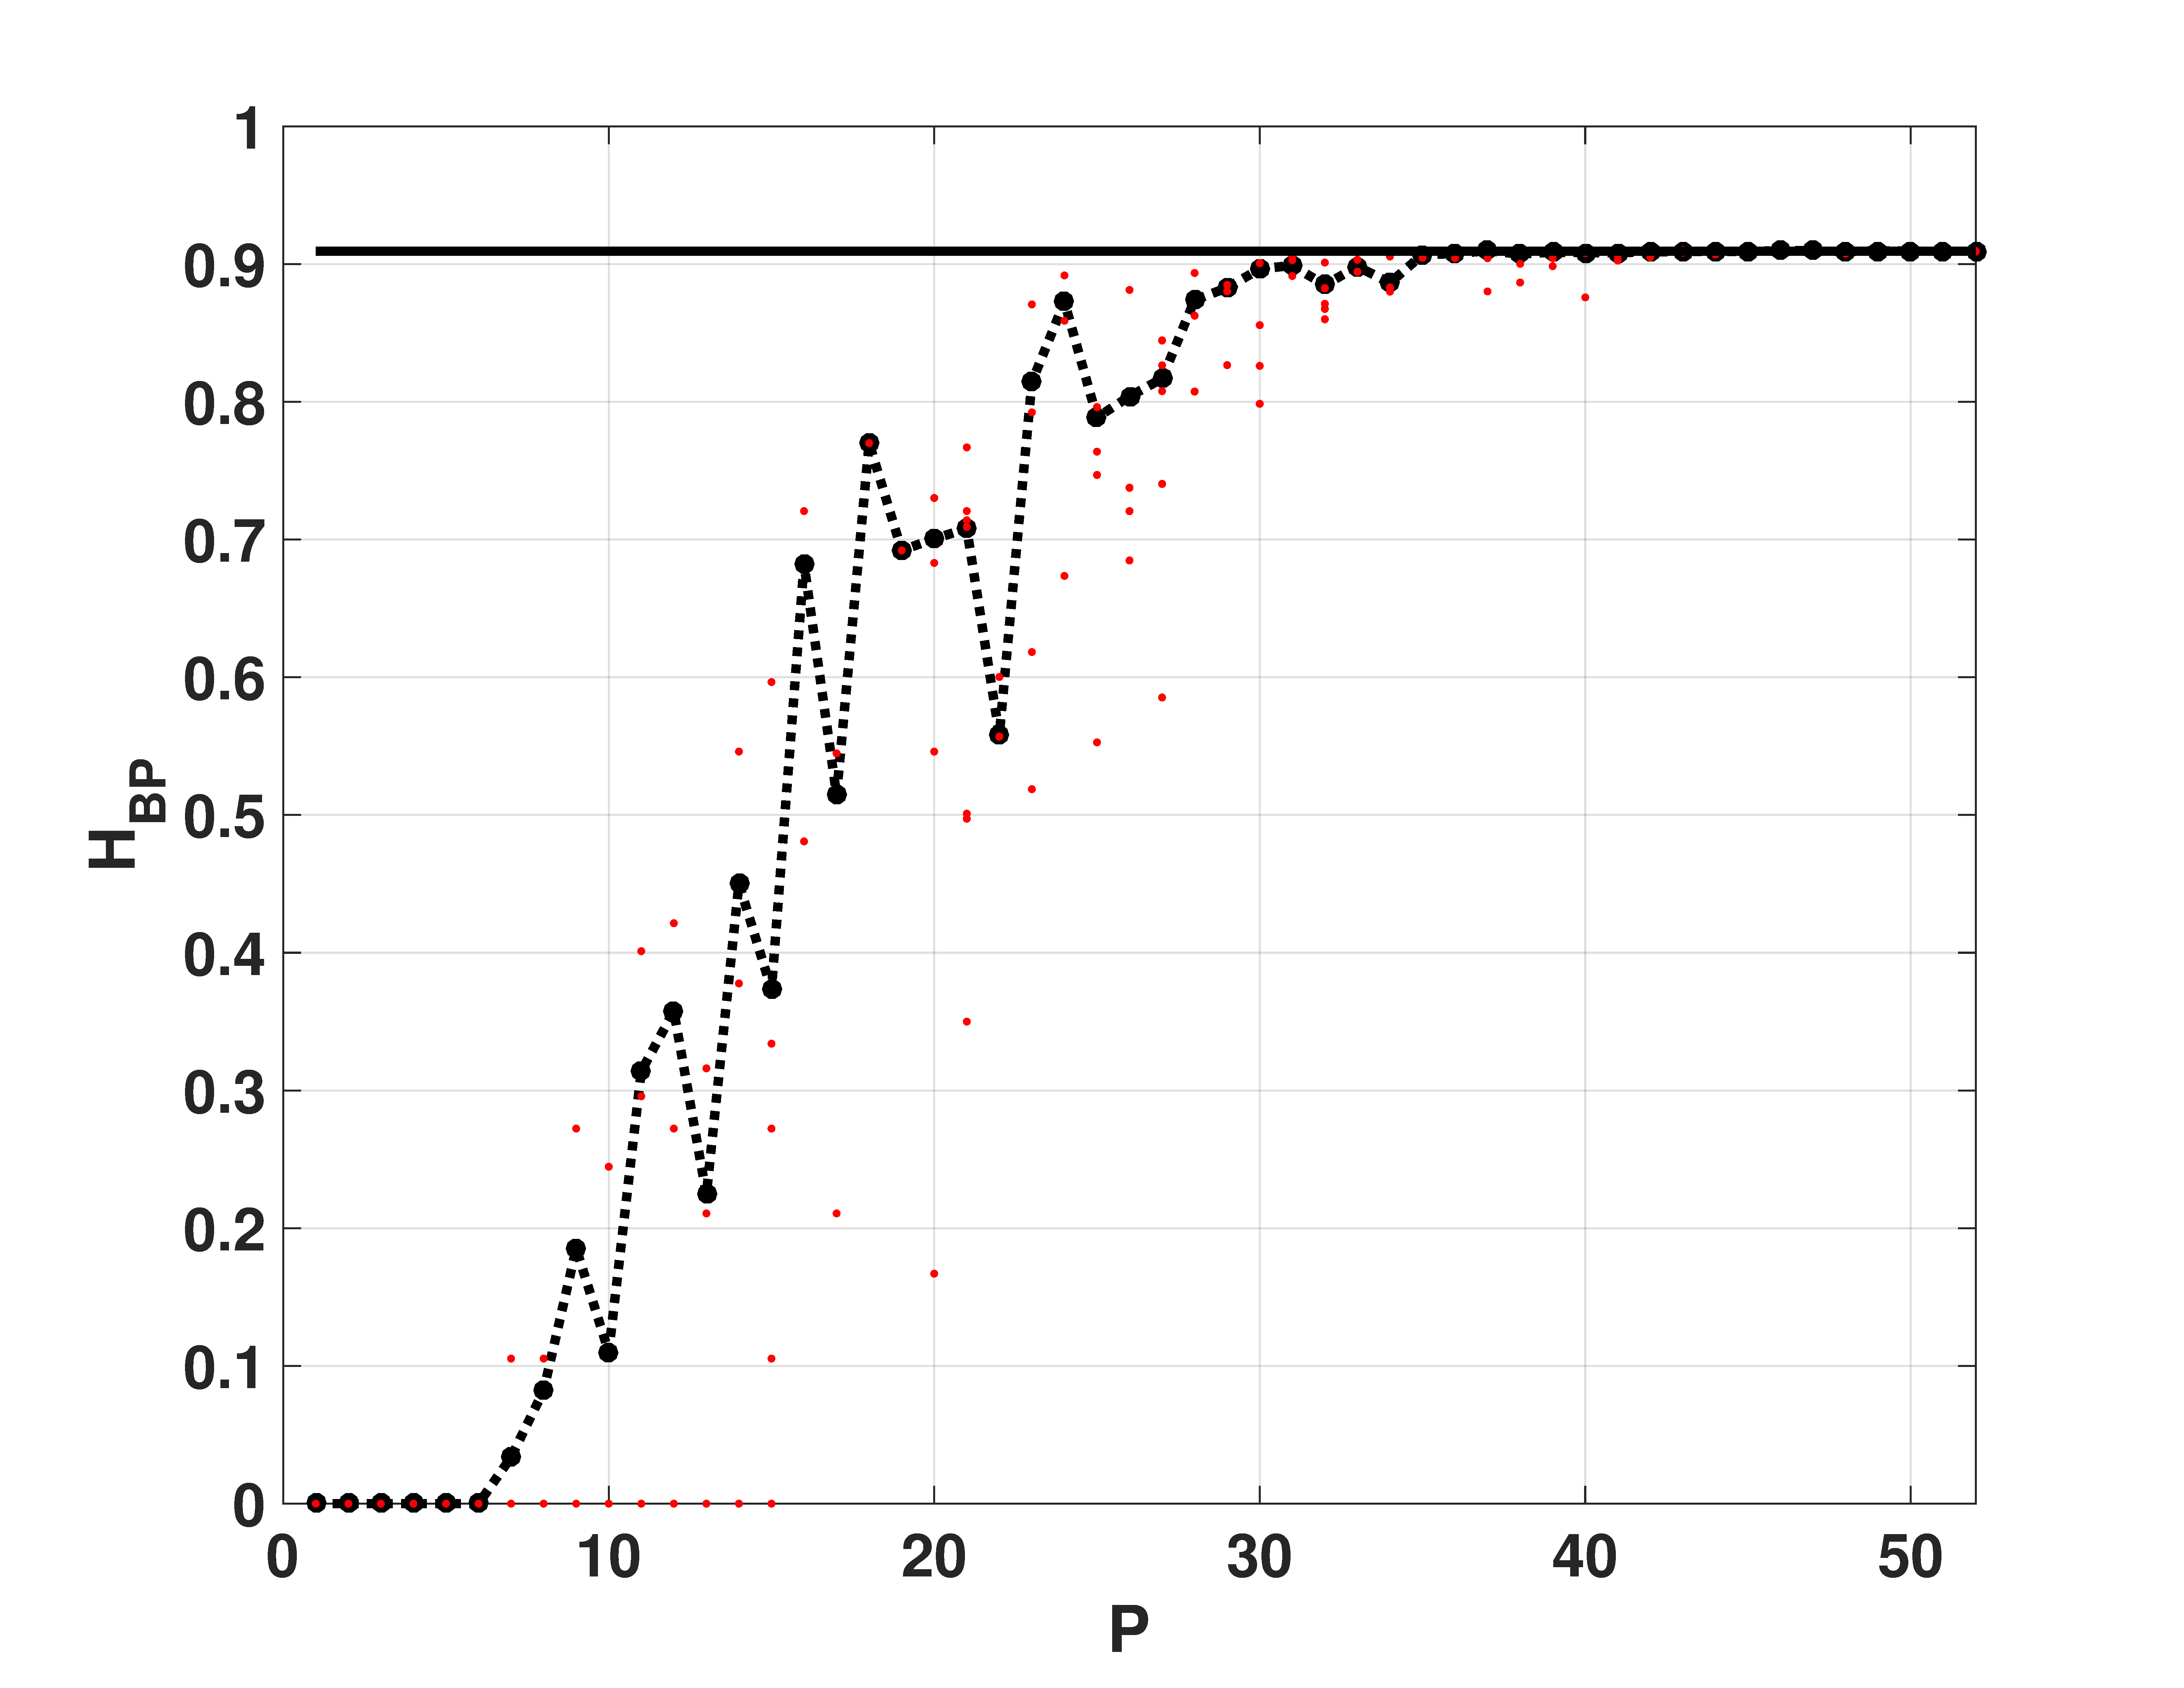
\includegraphics[width=\textwidth]{Hbp_Odd}
		\caption{$H_{BP}$ vs. $B$}
		\label{fig:Hbp_Odd}
	\end{subfigure}
	\begin{subfigure}[b]{0.49\textwidth}
		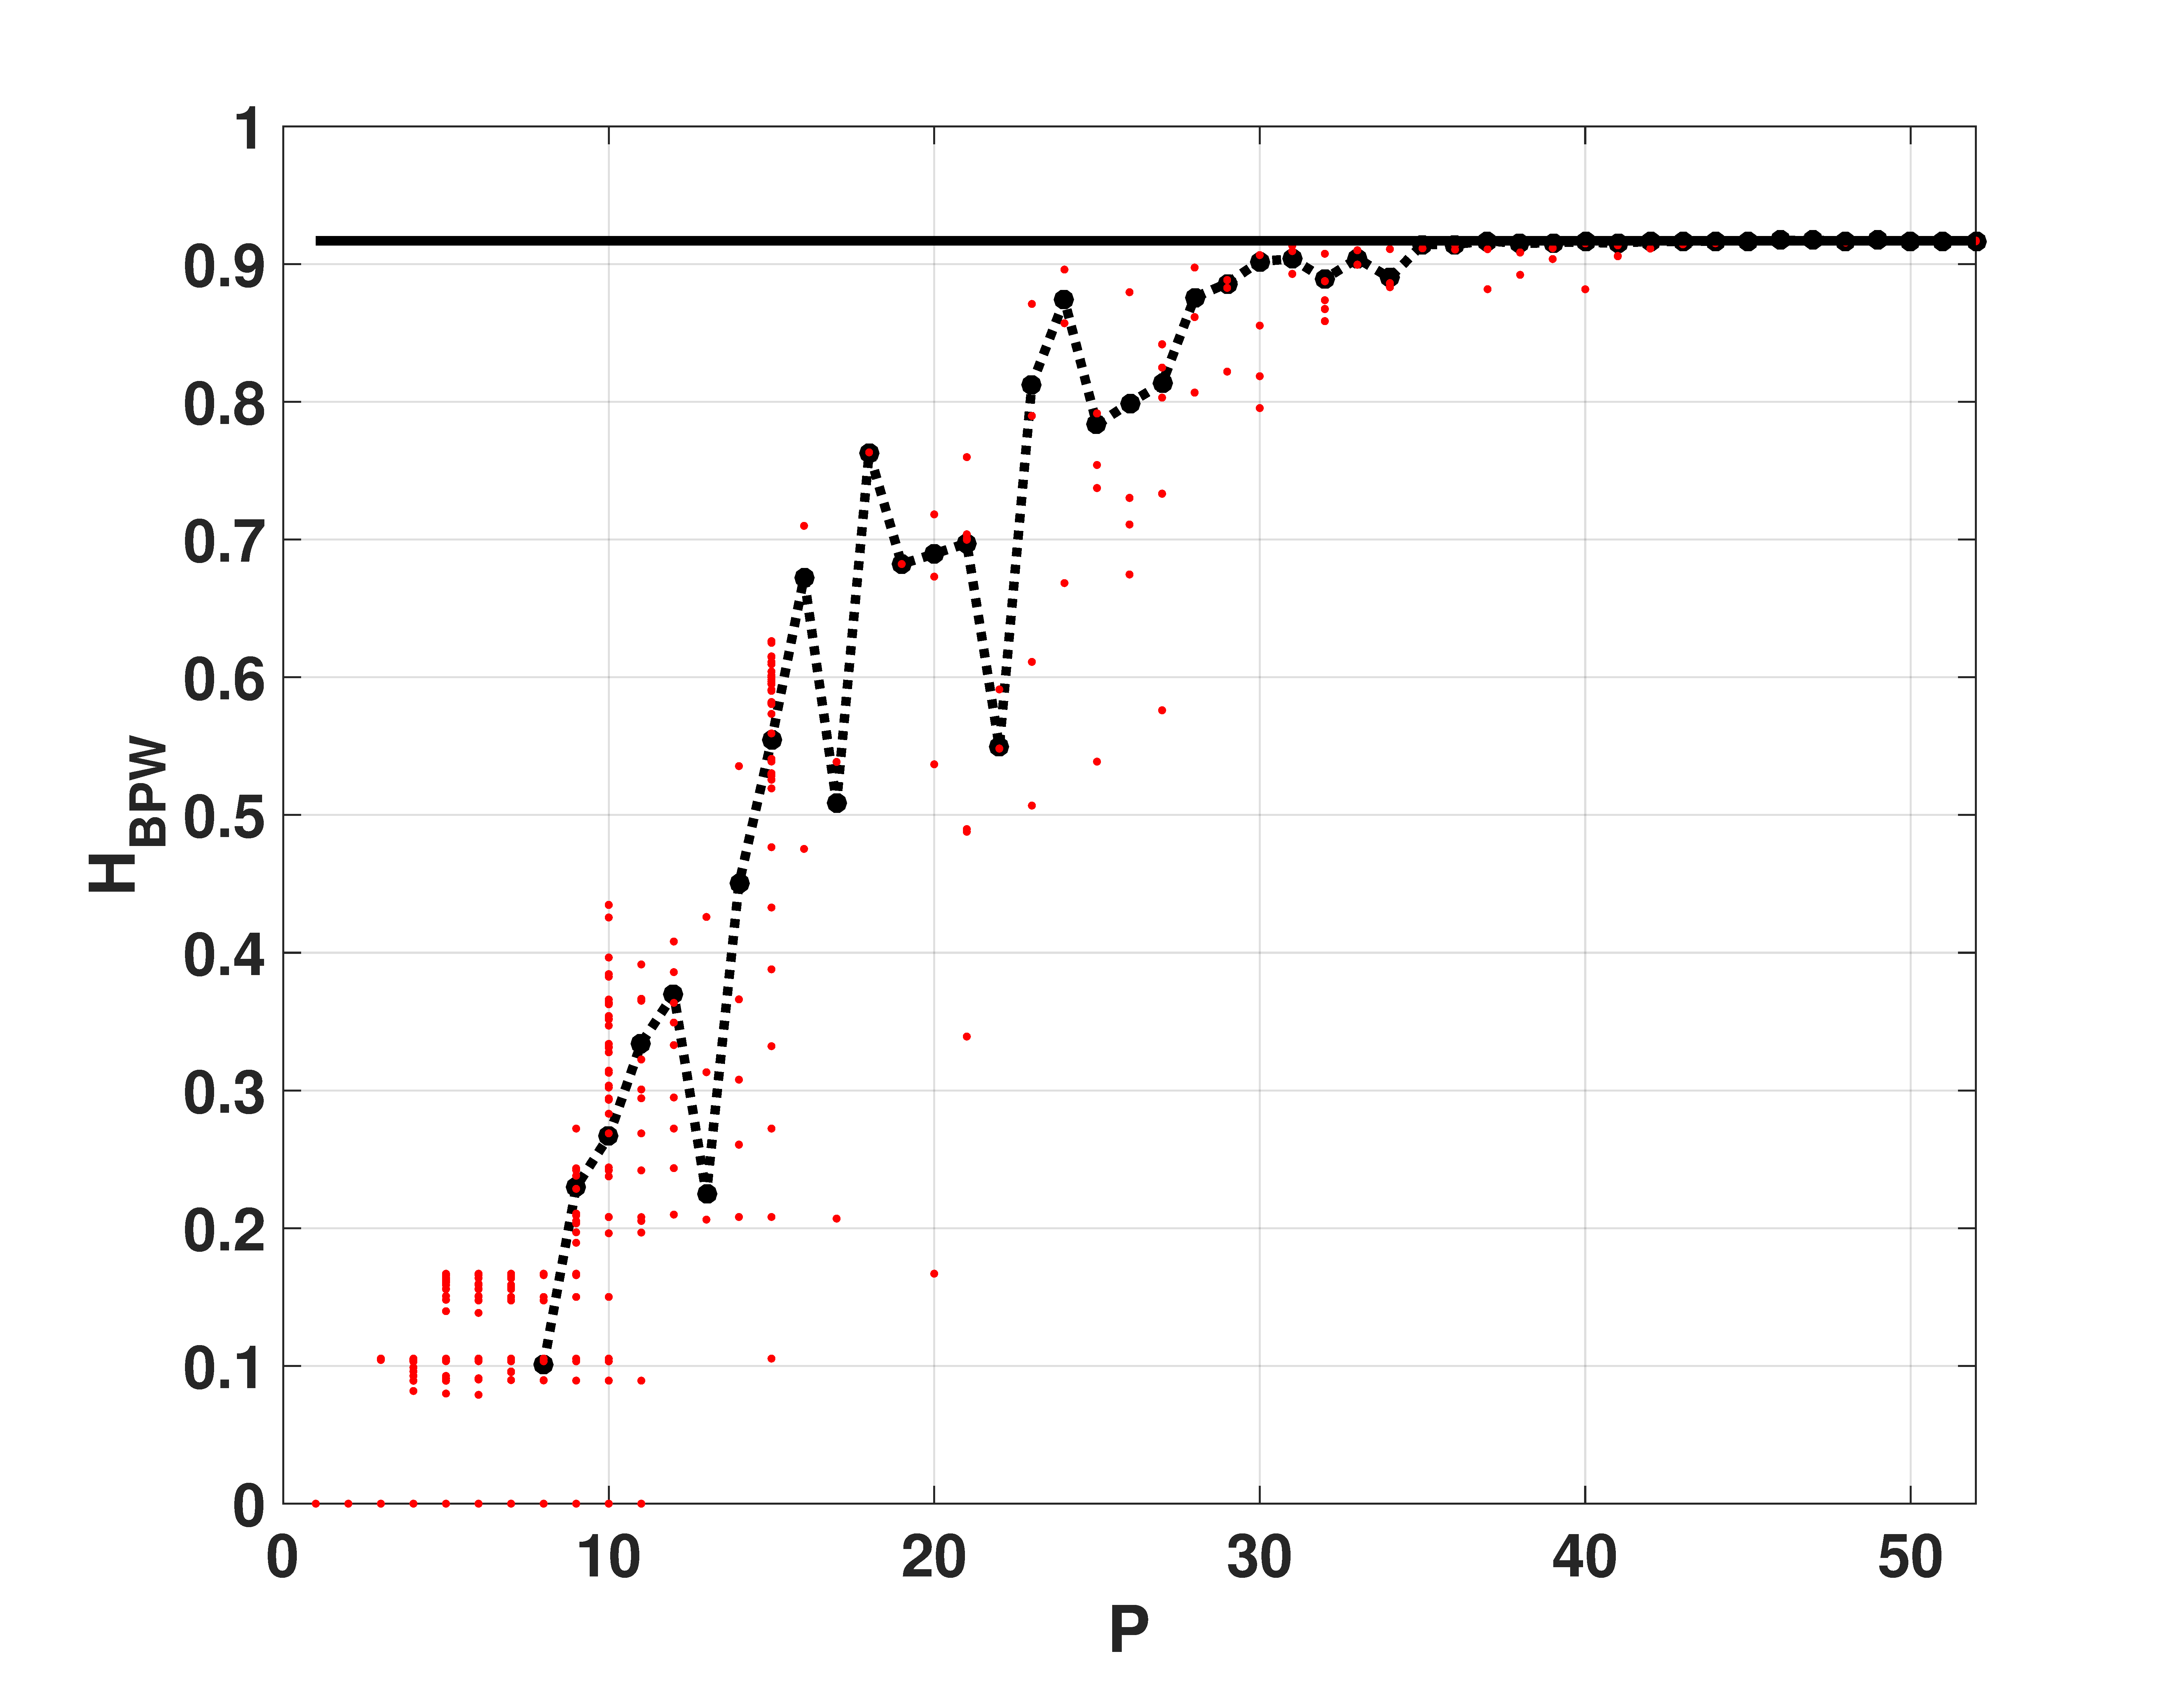
\includegraphics[width=\textwidth]{Hbpw_Odd}
		\caption{$H_{BPW}$ vs. $B$}
		\label{fig:Hbpw_Odd}
	\end{subfigure}
	\begin{subfigure}[b]{0.49\textwidth}
		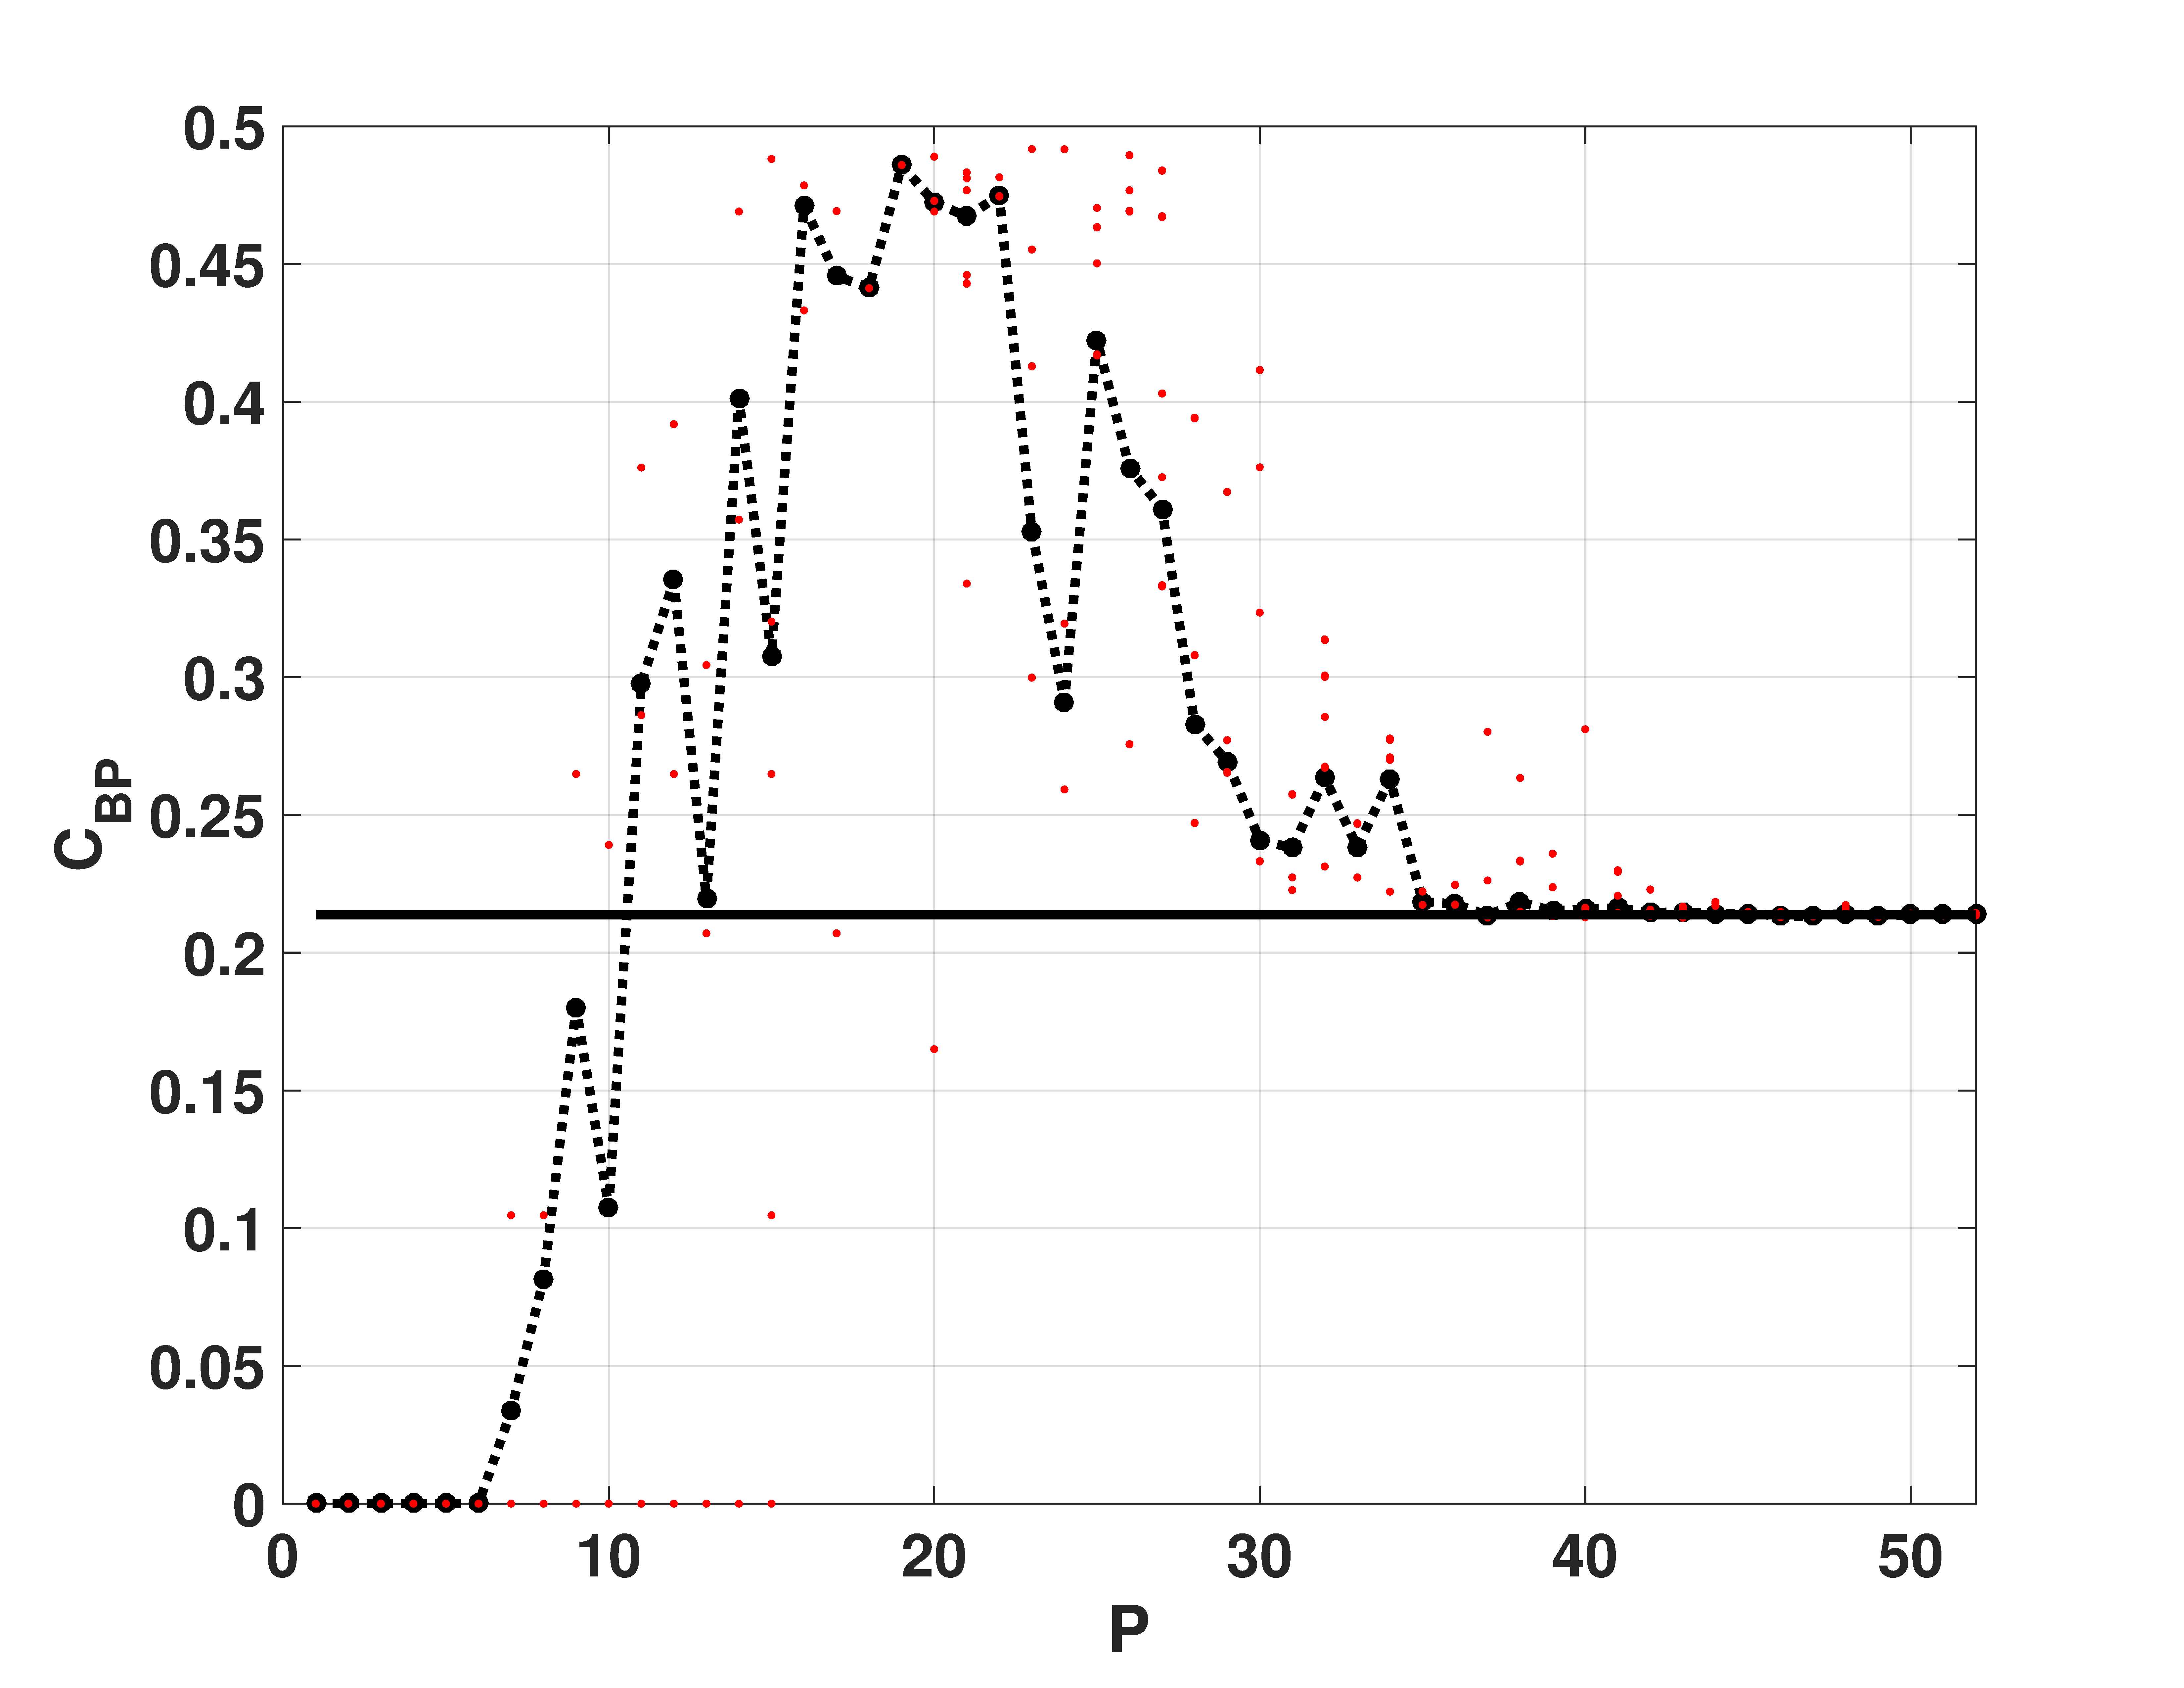
\includegraphics[width=\textwidth]{Cbp_Odd}
		\caption{$C_{BP}$ vs. $B$}
		\label{fig:Cbp_Odd}
	\end{subfigure}
	\begin{subfigure}[b]{0.49\textwidth}
		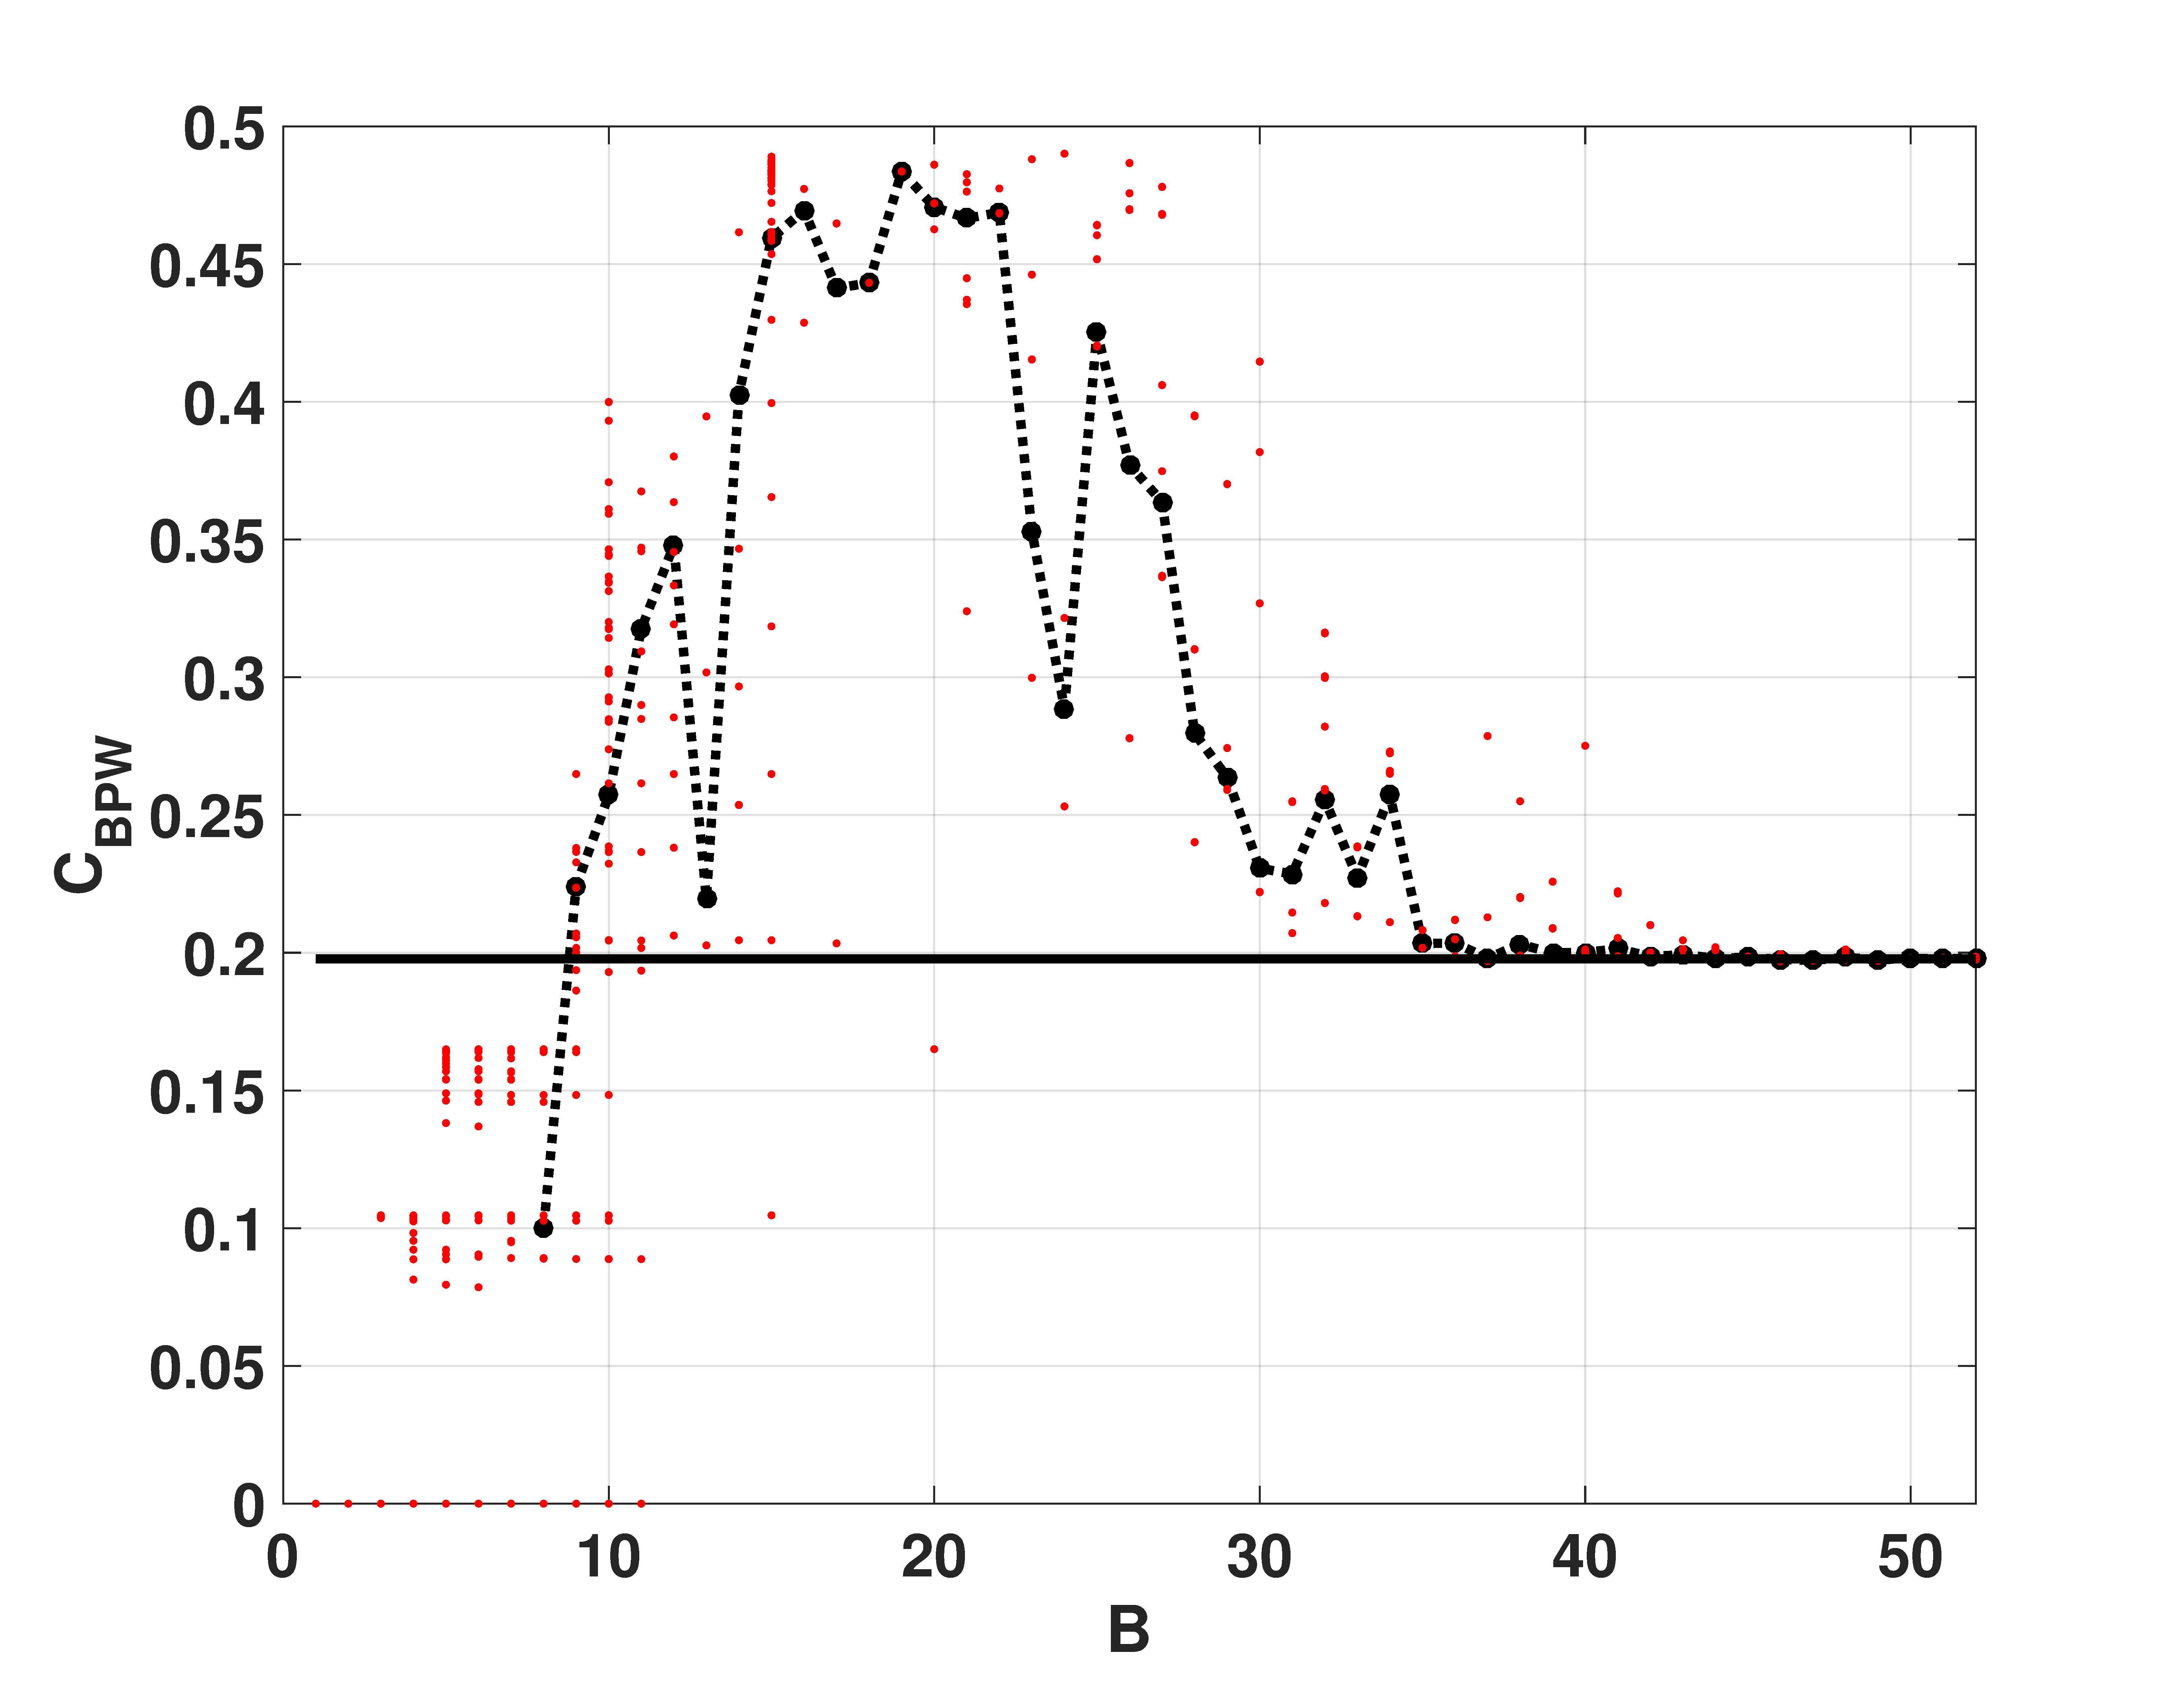
\includegraphics[width=\textwidth]{Cbpw_Odd}
		\caption{$C_{BPW}$ vs. $B$}
		\label{fig:Cbpw_Odd}
	\end{subfigure}
	\begin{subfigure}[b]{0.49\textwidth}
		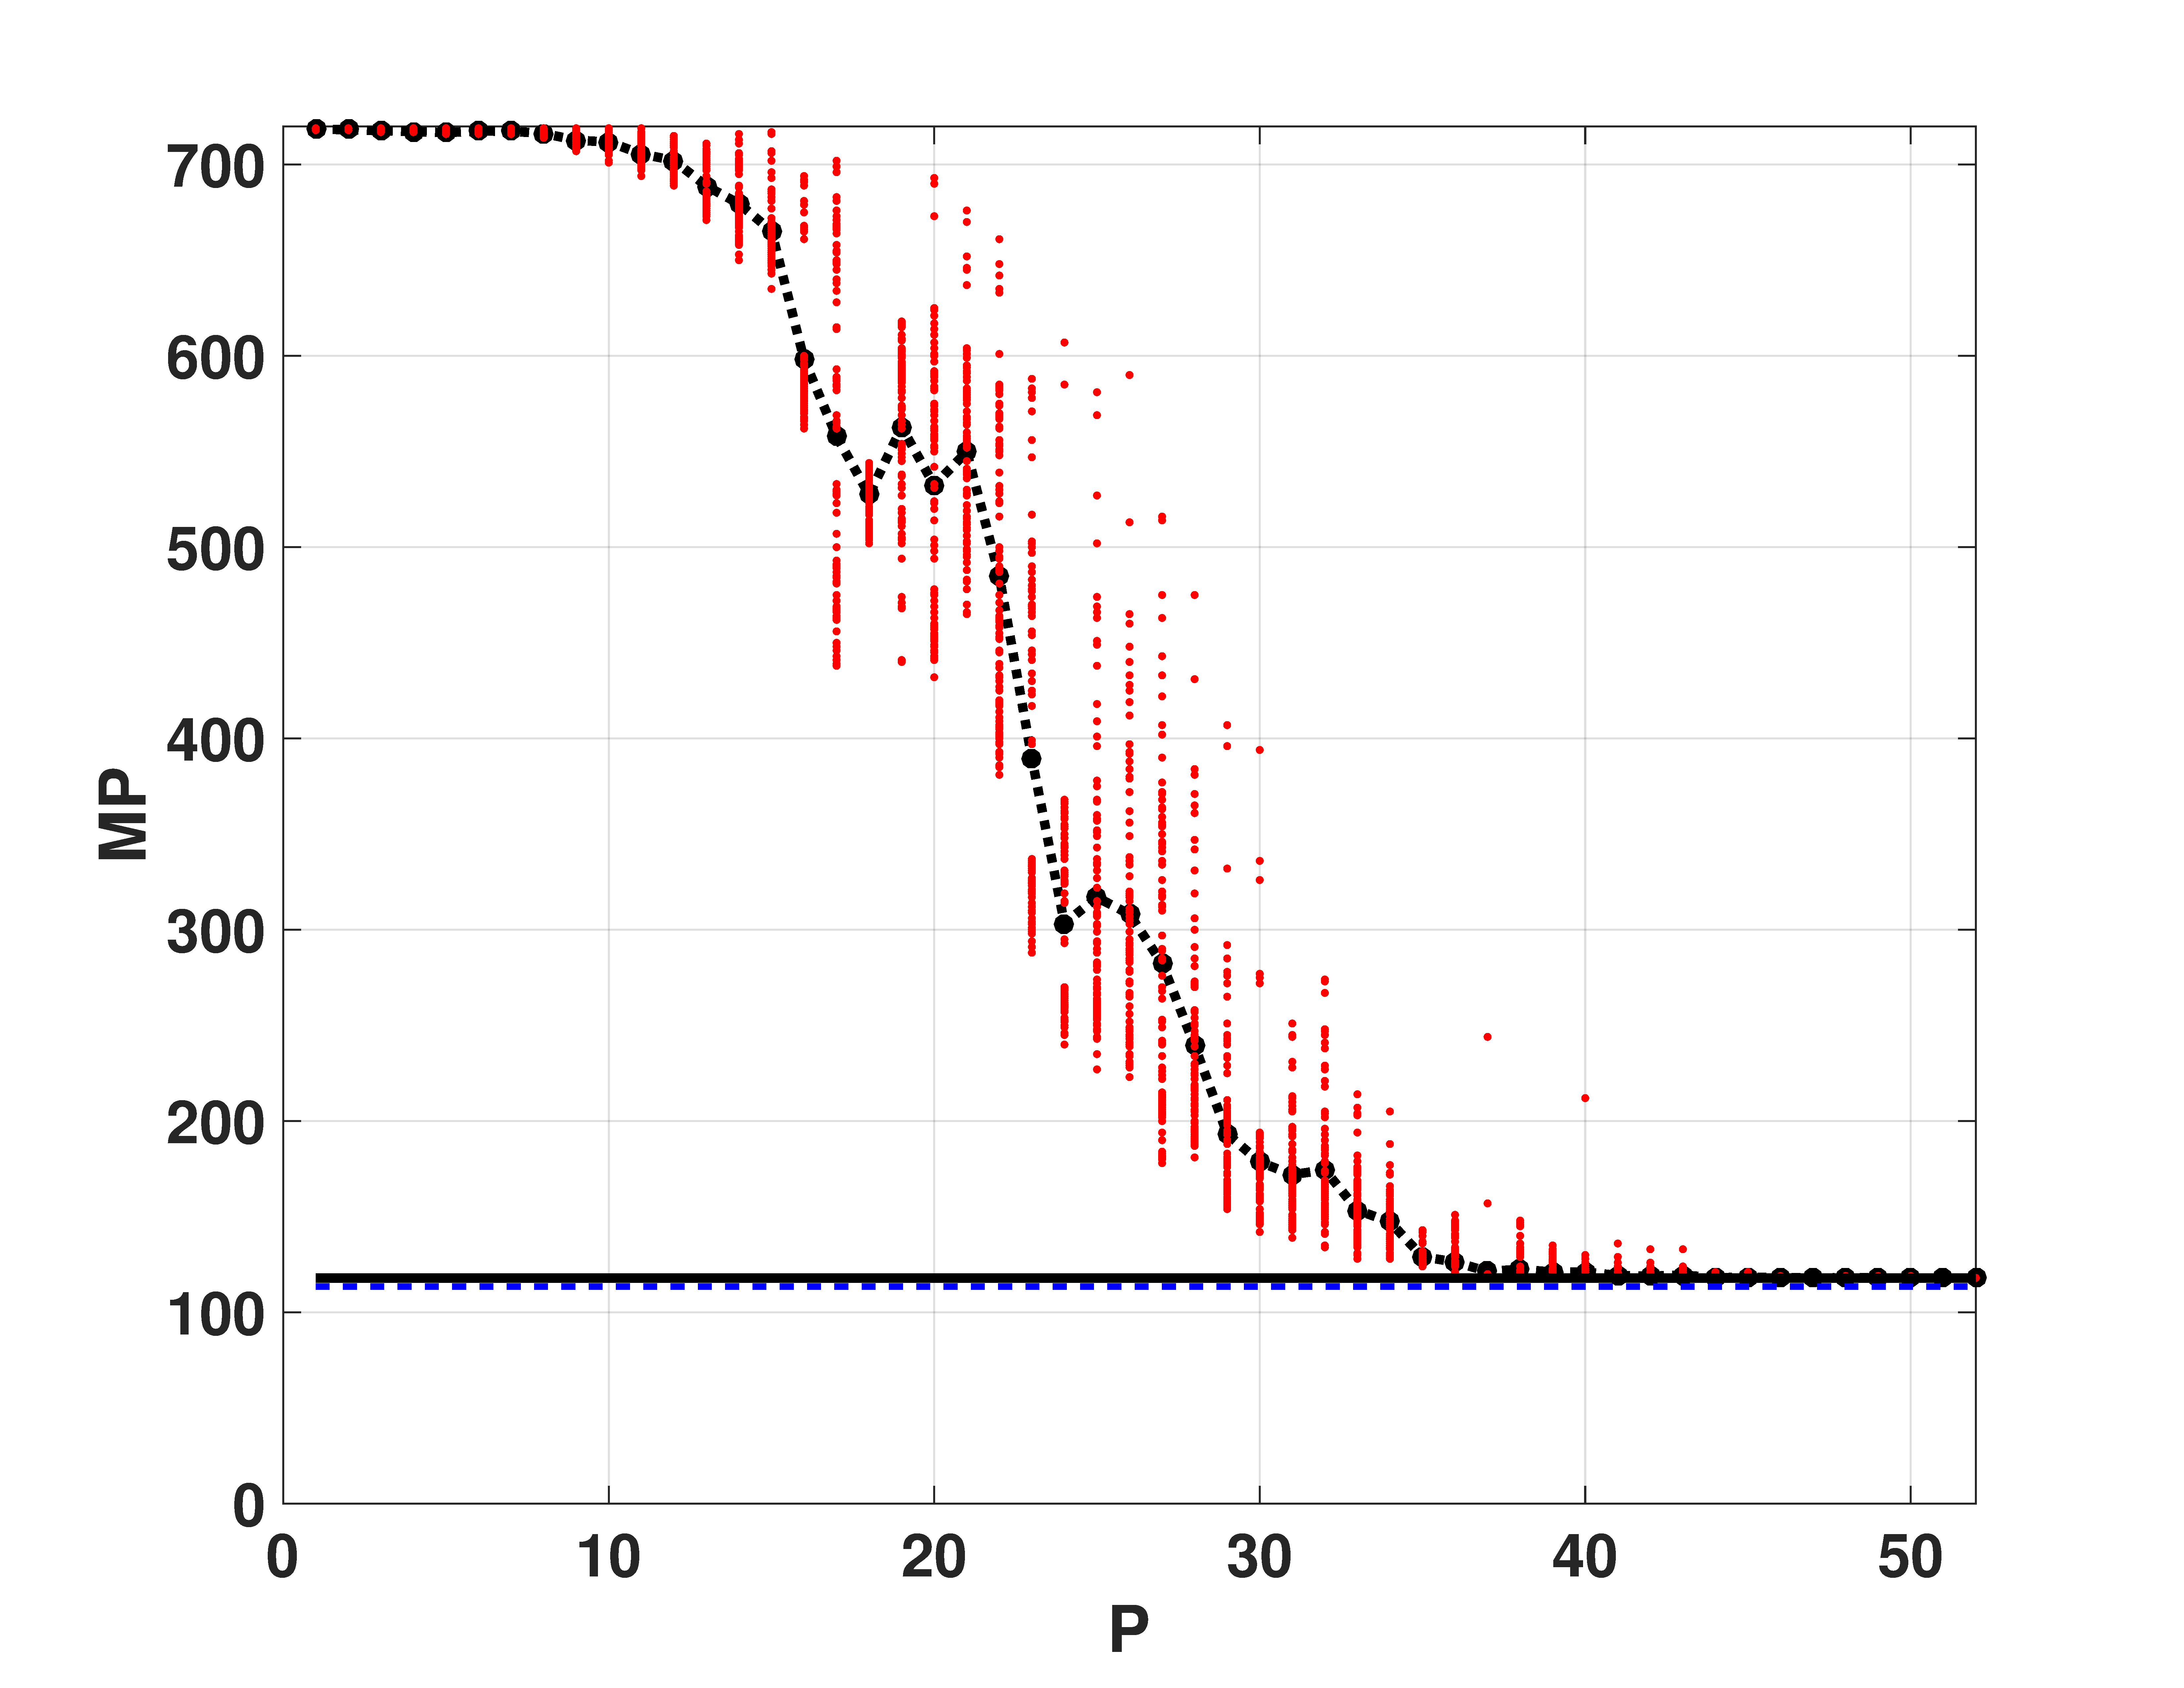
\includegraphics[width=\textwidth]{MP_Odd}
		\caption{MP vs. $B$}
		\label{fig:MP_Odd}
	\end{subfigure}
	\caption{Statistical properties of ODD map.}
	\label{fig:ODD_QuantiB}
\end{figure}

The enhancement showed in Fig. \ref{fig:EVEN_QuantiB} and \ref{fig:ODD_QuantiB} is reflected in the position of asymptotic point in the planes \ref{fig:EVEN_HH}, and \ref{fig:ODD_HH}.
In both cases this position is closest to the ideal point $(H_{hist}, H_{BP})=(1, 1)$, because the resulting vectors present better mixing.

\begin{figure}[H]
	\centering
	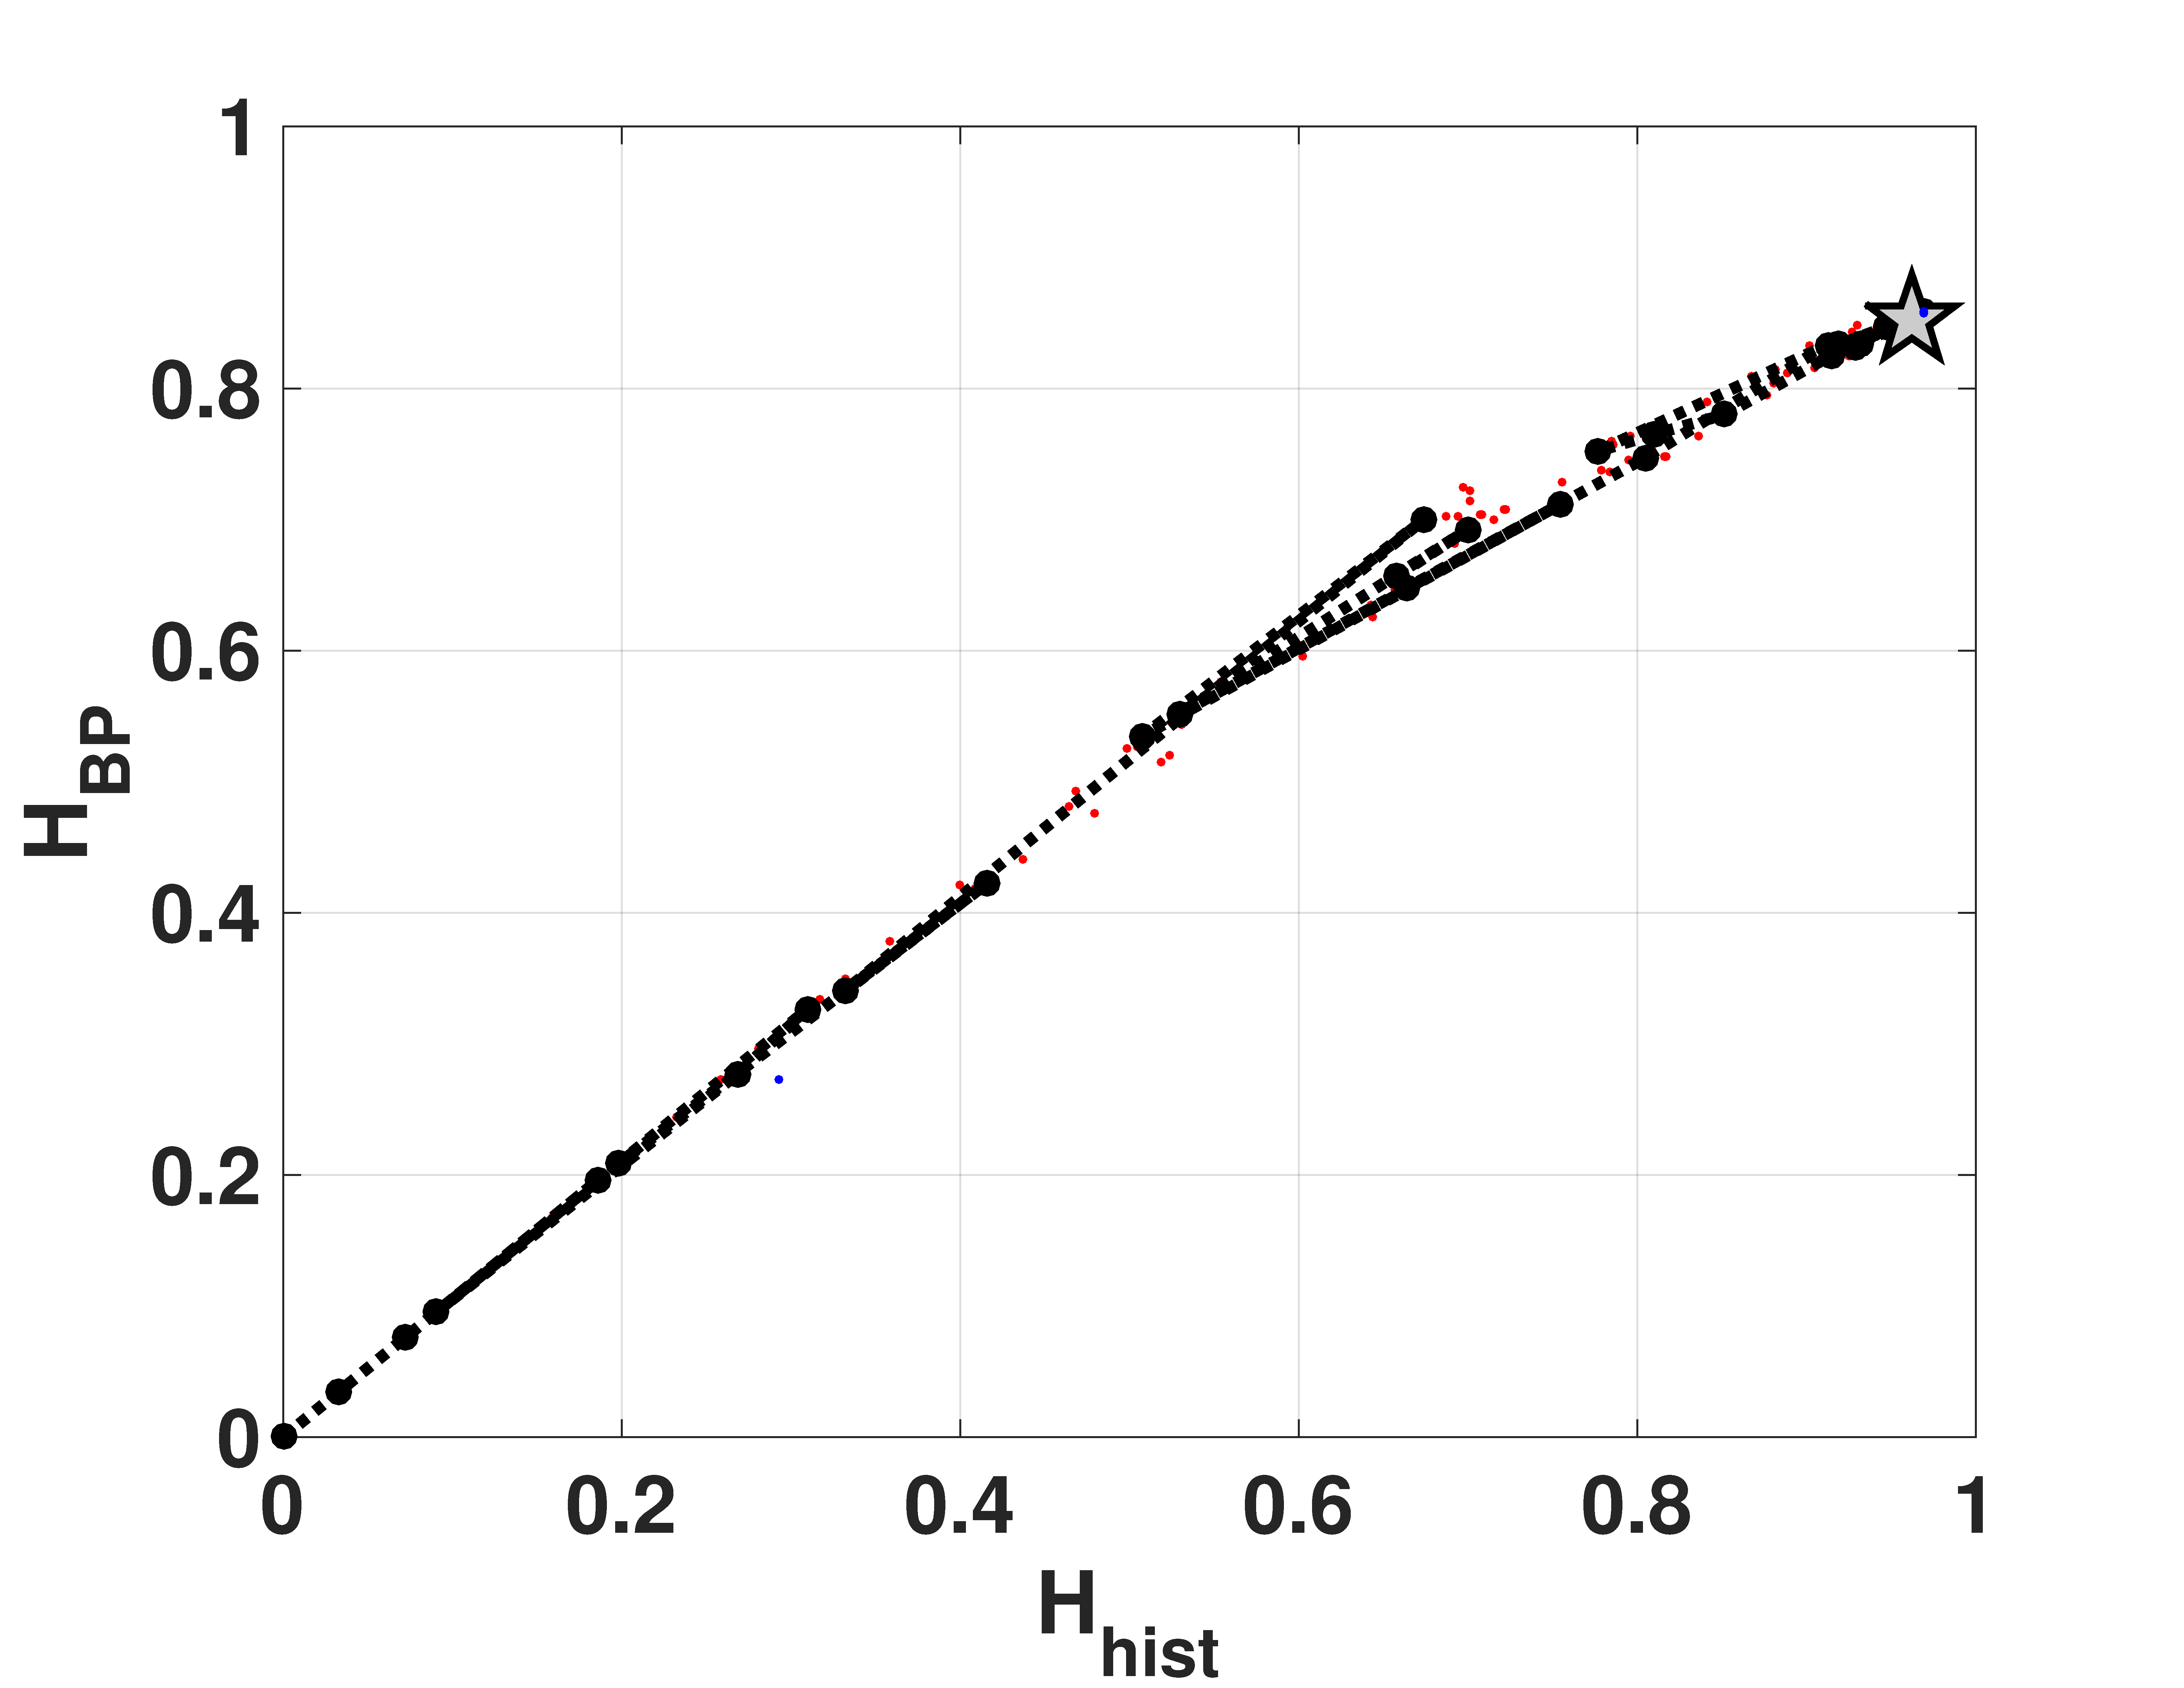
\includegraphics[width=.49\textwidth]{HbpHval_Even}
	\caption{Evolution of statistical properties in double entropy plane for EVEN map $H_{hist} \times H_{BP}$.}
	\label{fig:EVEN_HH}
\end{figure}

\begin{figure}[H]
	\centering
	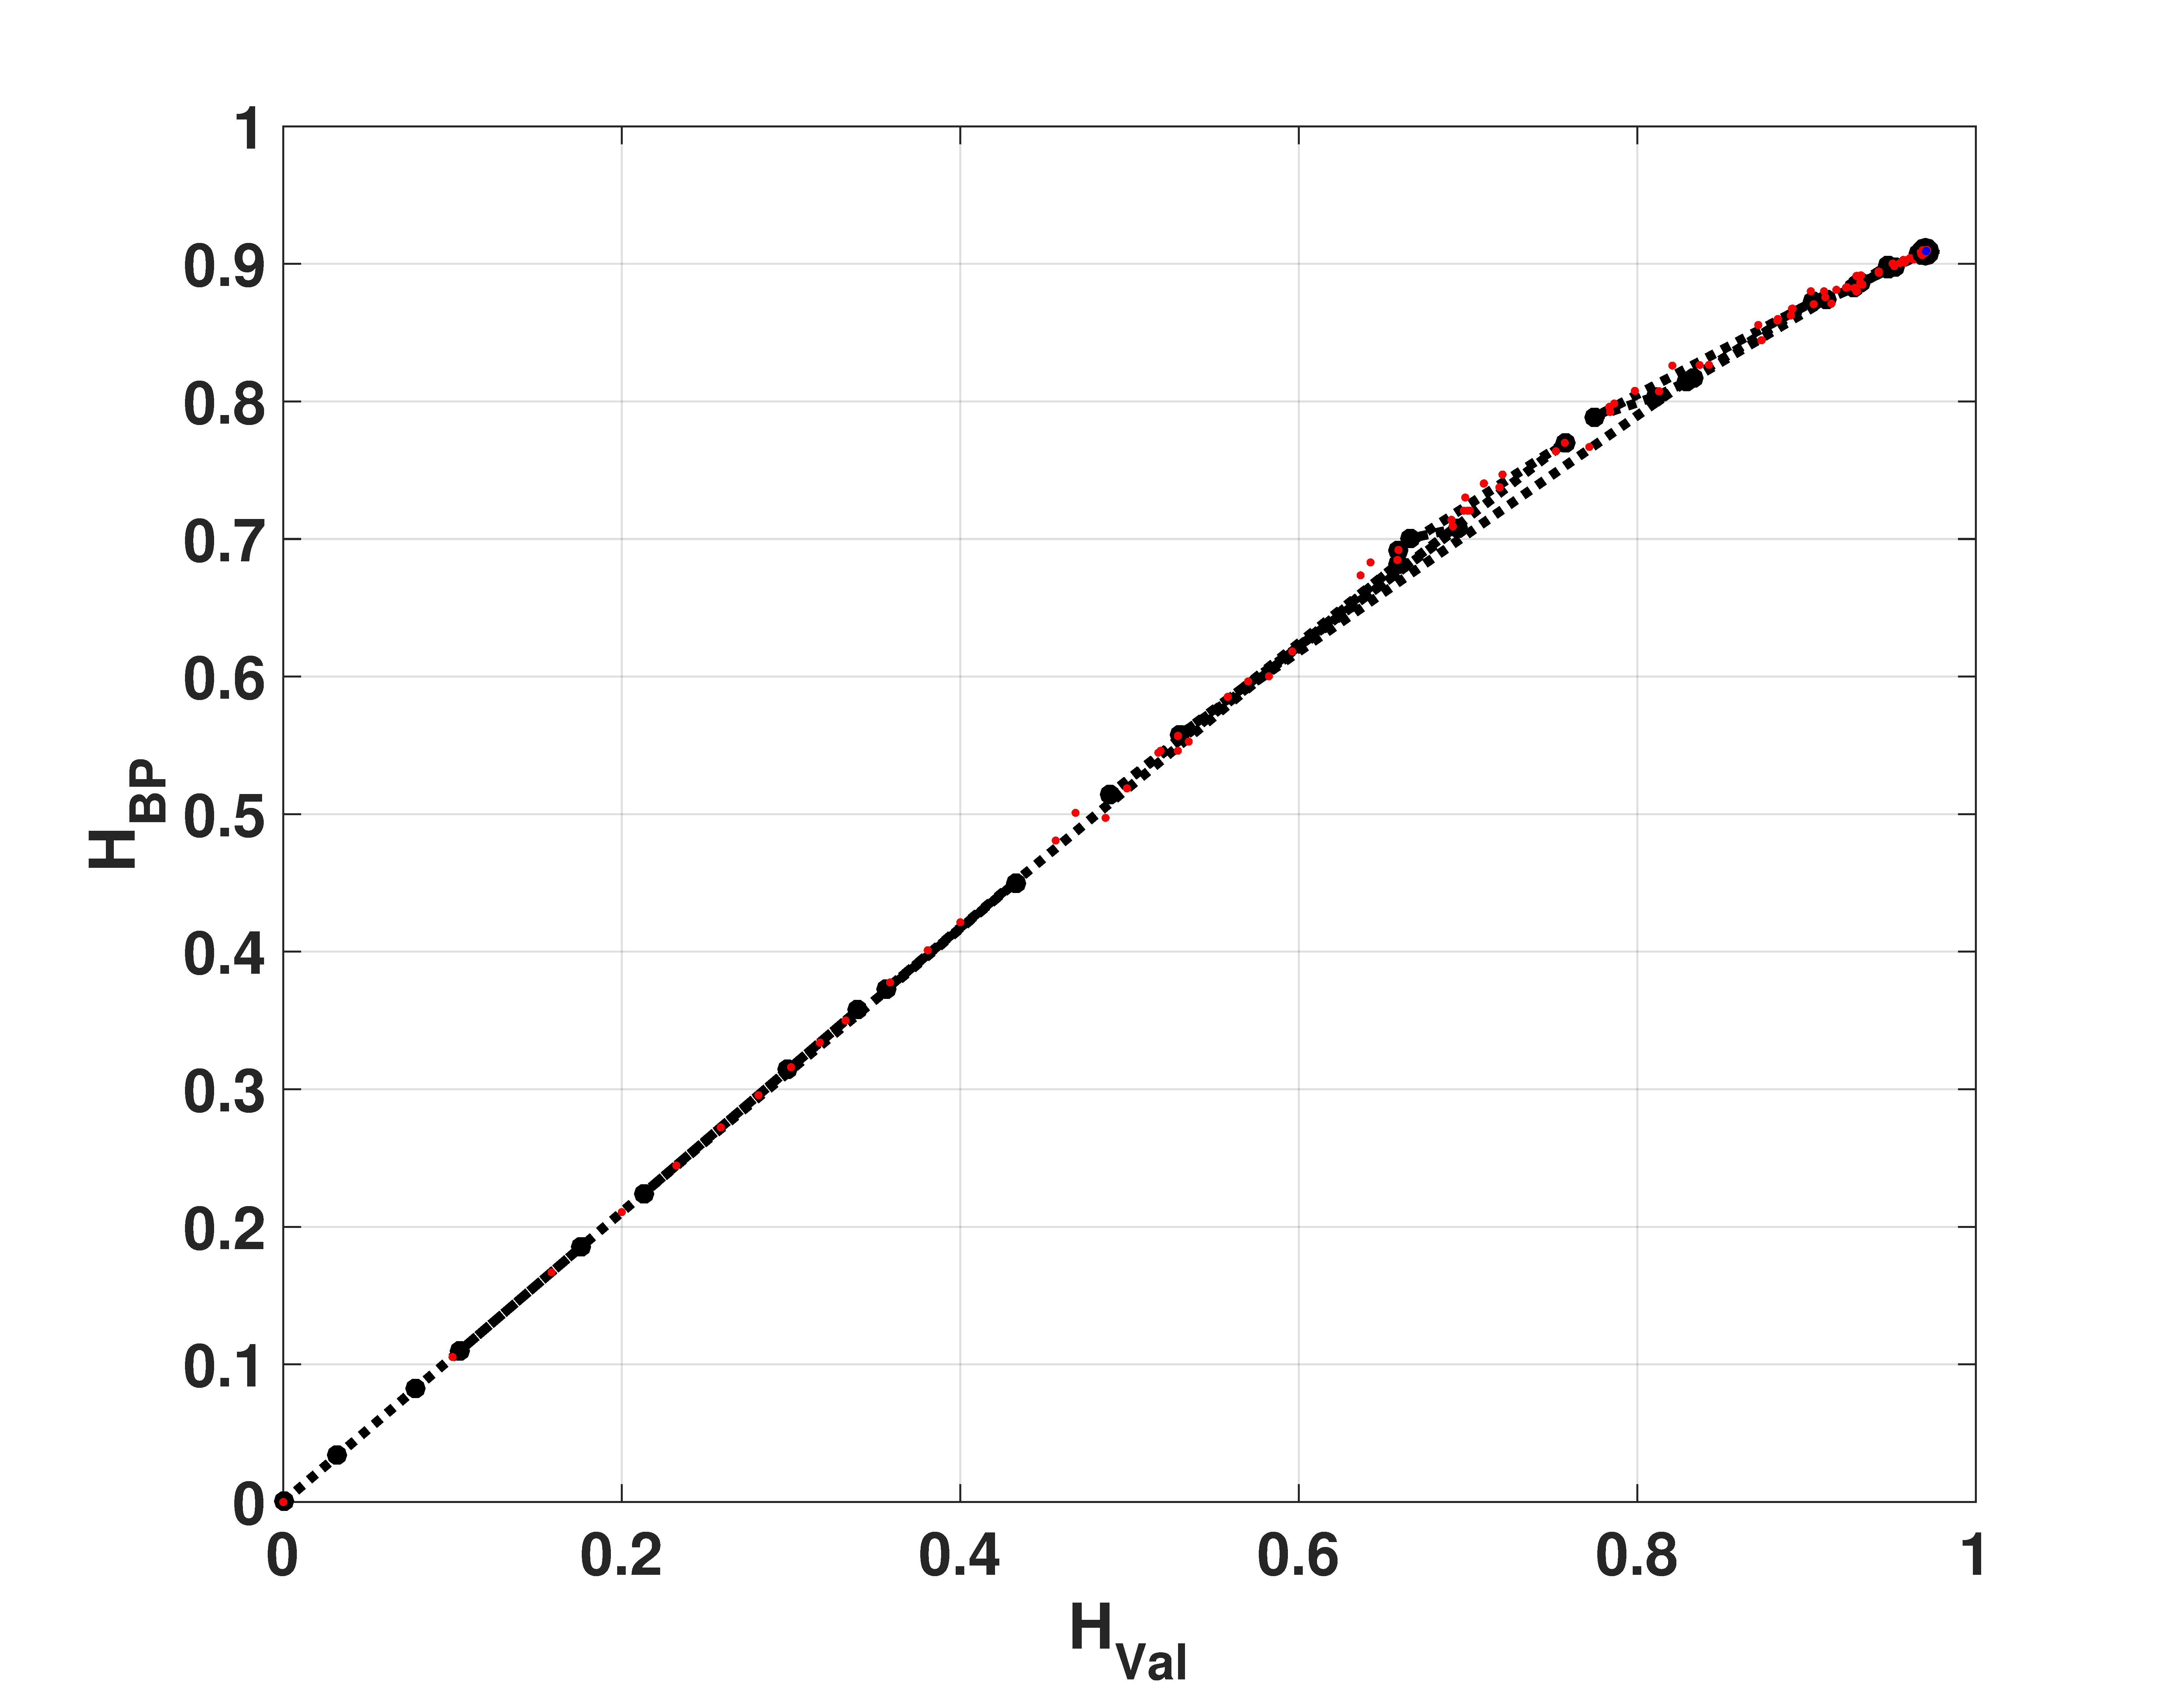
\includegraphics[width=.49\textwidth]{HbpHval_Odd}
	\caption{Evolution of statistical properties in double entropy plane for ODD map $H_{hist} \times H_{BP}$.}
	\label{fig:ODD_HH}
\end{figure}

Compatible results are shown in Figs. \ref{fig:EVEN_HC} and \ref{fig:ODD_HC}, the position of asymptotic point is closest to the ideal point $(H_{hist}, H_{BP})=(1, 0)$.
This result reflects that mixing is better because the complexity of resulting system is lower.
This plane detects that the vector generated by ODD skipping is more mixed than EVEN.
 
\begin{figure}[H]
	\centering
	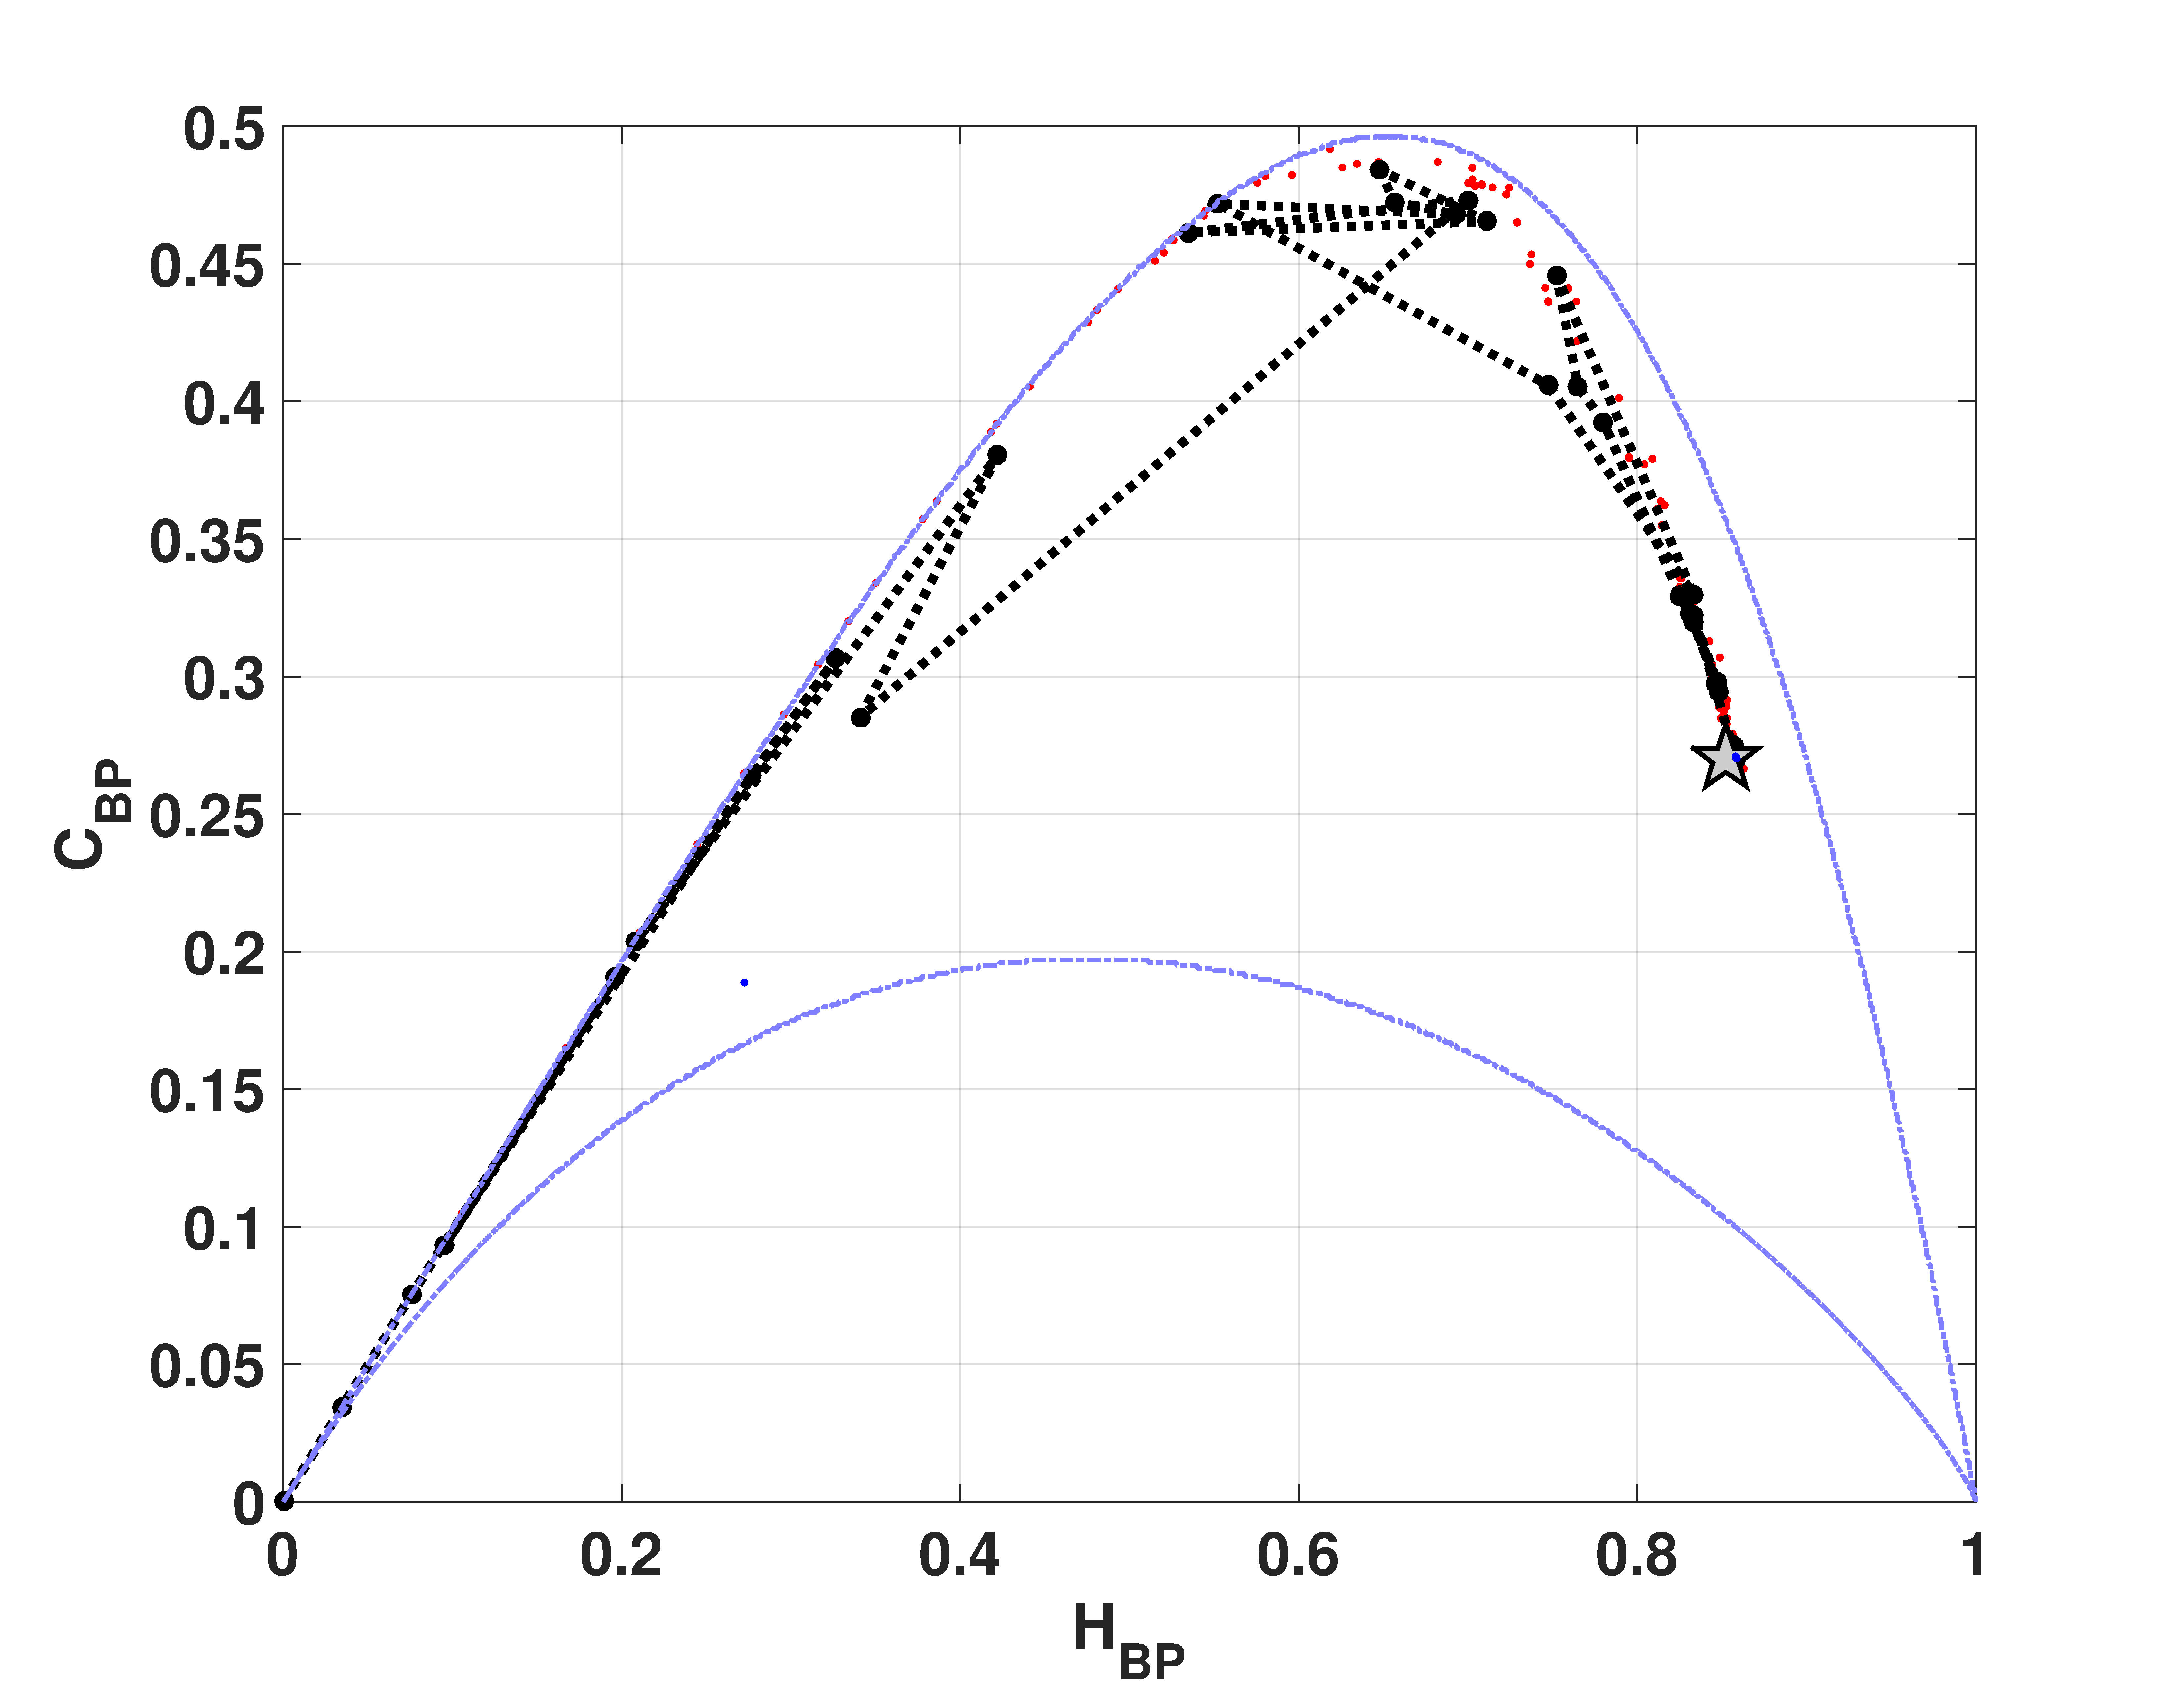
\includegraphics[width=.49\textwidth]{CbpHbp_Even}
	\caption{Evolution of statistical properties in entropy-complexity plane for EVEN map $H_{BP} \times C_{BP}$.}
	\label{fig:EVEN_HC}
\end{figure}

\begin{figure}[H]
	\centering
	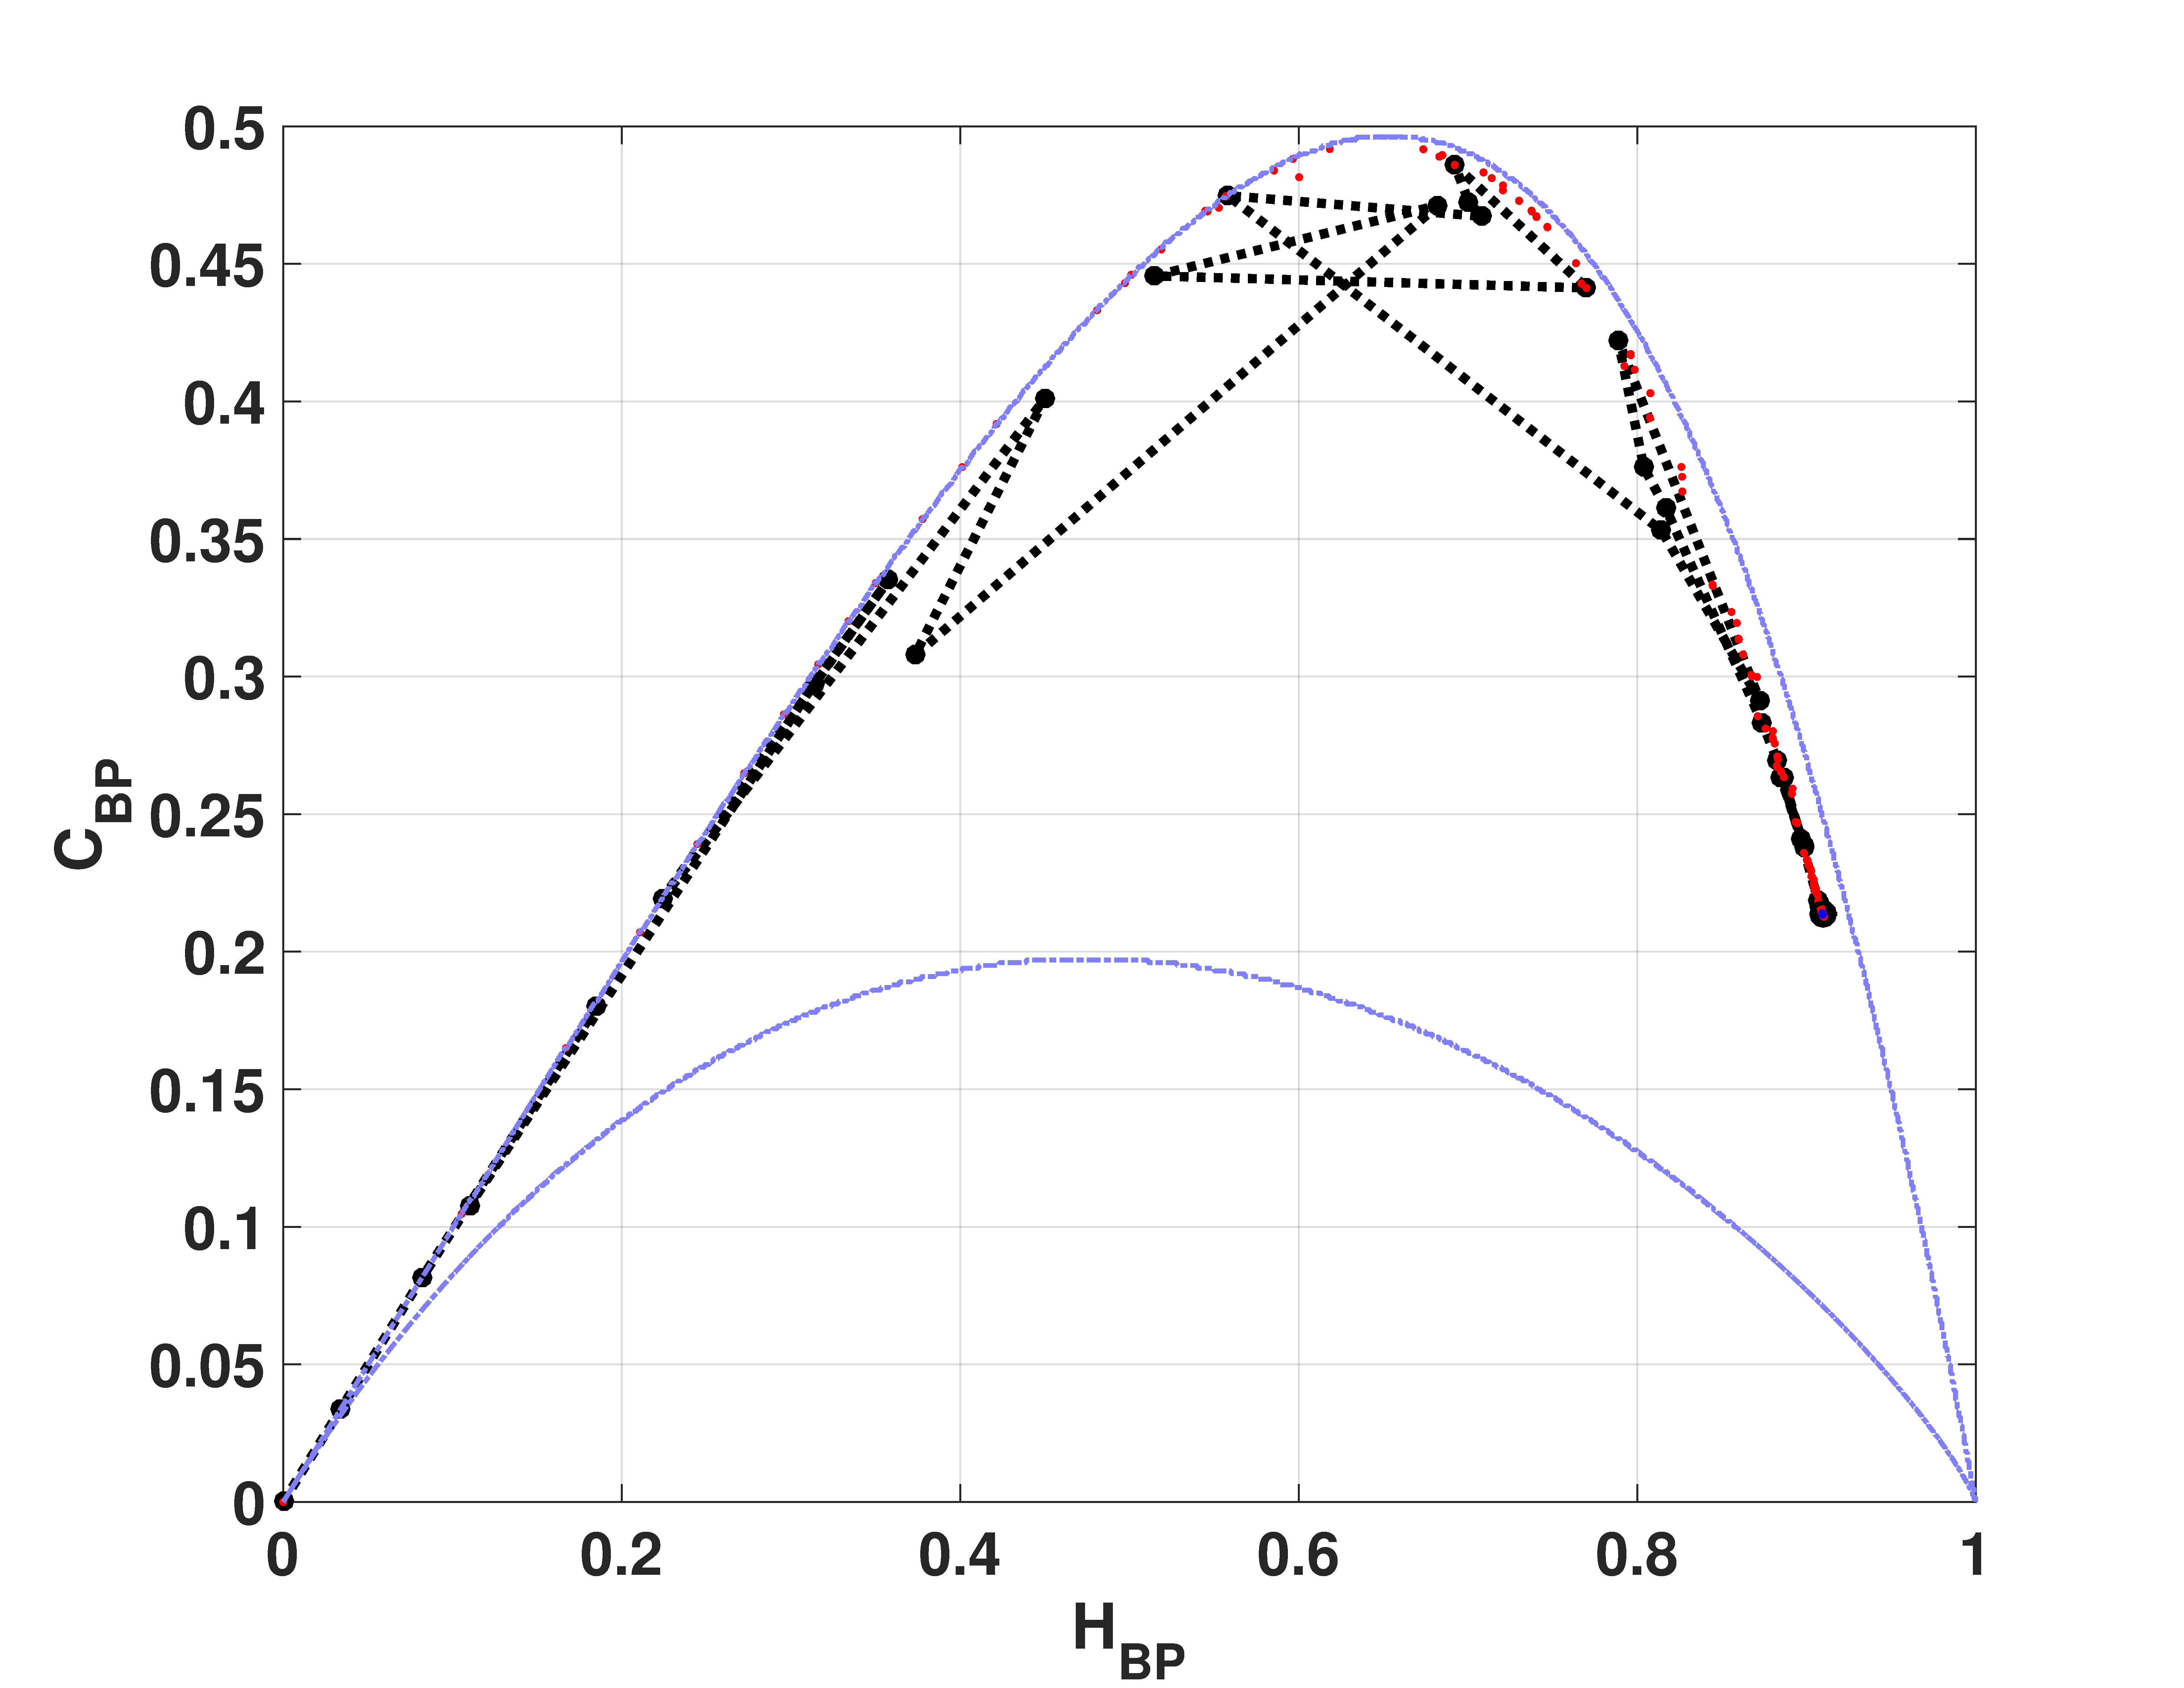
\includegraphics[width=.49\textwidth]{CbpHbp_Odd}
	\caption{Evolution of statistical properties in entropy-complexity plane for ODD map $H_{BP} \times C_{BP}$.}
	\label{fig:ODD_HC}
\end{figure}